\documentclass[11pt,a4paper]{article}

\usepackage[T1]{fontenc}
\usepackage[utf8]{inputenc}
\usepackage{lmodern}
\usepackage[margin=2.3cm]{geometry}
\usepackage{amsmath,amssymb,bm}
\usepackage{graphicx}
\usepackage{booktabs}
\usepackage{array}
\usepackage{tabularx}
\usepackage{xcolor}
\usepackage{tikz}
\usetikzlibrary{arrows.meta,positioning,calc,fit,backgrounds}
\usepackage{algorithm}
\usepackage{algpseudocode}
\usepackage{caption}
\usepackage{float}
\usepackage{enumitem}
\usepackage{listings}
\usepackage{url}
\usepackage[hidelinks]{hyperref}

\graphicspath{{figures/}}

\definecolor{codebg}{HTML}{F5F5F2}
\definecolor{psogreen}{HTML}{1BAF7A}
\definecolor{pdblue}{HTML}{2A78D6}
\definecolor{accent}{HTML}{EB6834}
\definecolor{violet}{HTML}{6250D6}
\lstset{basicstyle=\ttfamily\small, backgroundcolor=\color{codebg}, frame=single, rulecolor=\color{gray!40},
        columns=fullflexible, keepspaces=true, xleftmargin=4pt, xrightmargin=4pt, aboveskip=8pt, belowskip=8pt}
\lstdefinestyle{py}{language=Python, basicstyle=\ttfamily\footnotesize, keywordstyle=\bfseries,
        numbers=left, numberstyle=\tiny\color{gray}, numbersep=6pt, xleftmargin=18pt}

\newcommand{\code}[1]{\texttt{\detokenize{#1}}}
\DeclareUrlCommand\file{\urlstyle{tt}}
\newcommand{\sgn}{\operatorname{sign}}
\newcommand{\sat}{\operatorname{sat}}
\newcommand{\clip}{\operatorname{clip}}

\setlength{\parskip}{4pt}
\setlength{\emergencystretch}{2.5em}
\renewcommand{\arraystretch}{1.15}
\captionsetup{font=small, labelfont=bf}

\title{\textbf{Particle Swarm Optimisation for Automatic PID Tuning\\of the Geomagic Touch (Phantom Omni)}\\[6pt]
\large Algorithm, application, swarm behaviour, results and usage}
\author{}
\date{\today}

\begin{document}
\maketitle

\begin{abstract}
This document presents the use of Particle Swarm Optimisation (PSO) to tune, automatically, the three
joint PID controllers of the Geomagic Touch (Phantom Omni) haptic robot. It explains the PSO algorithm
and every design choice in its implementation (decreasing inertia weight, coefficient safeguard, velocity
clamping, reflective boundaries), then shows how a PID tuning problem is turned into something a swarm
can solve: each particle is a vector of nine gains, and its fitness is obtained by simulating the robot's
joints and scoring the response for accuracy, torque use and stability margins under a local loop and a
$20\,\mathrm{ms}$ network delay. The behaviour of the swarm is analysed from the inside (diversity,
share of unstable particles, evolution of the global best) and over ten random seeds. Starting from the
hand-designed PD controller of the thesis (cost $18.54$), PSO reached costs between $0.77$ and $1.08$ in
all ten runs, a $17$--$24$-fold improvement. The reference run produces PID gains that settle in about
$0.24\,\mathrm{s}$, leave less than $0.3^\circ$ of steady-state error (instead of $3.6$--$7.8^\circ$) and
reduce the Cartesian error on a seam-welding path from $33.8\,\mathrm{mm}$ to $2.2\,\mathrm{mm}$ RMS
($0.73\,\mathrm{mm}$ when PSO also tunes a task-space velocity controller). The final section explains
how to run everything.
\end{abstract}

\tableofcontents
\newpage

%=====================================================================================================
\section{Introduction}
%=====================================================================================================

\subsection{Context}

This work implements the milestone \emph{``Adaptive Control and Automatic Retuning''} from Section~7.9 of
the bachelor's thesis \emph{``Omni Bundle -- Haptic Device's Industrial Approach''}
\cite{gavan2026}. The thesis tunes the joint controllers of the Phantom Omni by hand:
\begin{itemize}[nosep]
  \item a \textbf{frequency-domain PD design}, used in simulation, which places the gain crossover at
        $\omega_c = 35\,\mathrm{rad/s}$ with a phase margin of $70^\circ$;
  \item a \textbf{manually tuned PID} on the QUARC real-time platform, available for joint~1 only.
\end{itemize}
The PD design has no integral action, so friction and gravity leave each joint $3^\circ$--$8^\circ$ short of
its target. The manual PID removes most of that error, but its phase margin is small, and it oscillates
strongly when the feedback travels over a UDP network.

\subsection{The tuning problem}

Each of the three joints has a PID controller with gains $K_p$, $K_i$, $K_d$, so the designer has to choose
nine numbers. A good choice must at the same time track a step quickly, without overshoot and without
steady-state error, stay within the motor torque ratings, and keep enough phase and delay margin to remain
stable when the loop is closed over a network. These goals conflict. Moreover, the quality of a set of
gains can only be measured by simulating the robot, and the result is neither smooth nor differentiable:
crossing a stability boundary turns a good response into a diverging one. Gradient-based optimisation is
therefore a poor fit.

\subsection{Why Particle Swarm Optimisation}

PSO \cite{kennedy1995} is a population-based, derivative-free global optimiser. It suits this problem well:
\begin{itemize}[nosep]
  \item it needs only the cost value of a candidate, never a gradient, so a simulation-based,
        discontinuous cost with penalty terms is no obstacle;
  \item a whole swarm explores the search space at once, so it is less likely than a local method to get
        stuck near the starting design;
  \item it has few parameters (swarm size, inertia, two acceleration coefficients), all with an intuitive
        meaning;
  \item all particles are evaluated independently, so the whole swarm can be simulated in one vectorised
        computation.
\end{itemize}
This document concentrates on PSO. The repository also contains a genetic algorithm
(\file{src/optimizers/ga.py}, selected with \code{--method ga}) as an alternative optimiser, which is not
discussed here.

\subsection{Structure of the document}

Section~\ref{sec:pso} explains the PSO algorithm and its implementation. Section~\ref{sec:application}
shows how PID tuning is encoded for the swarm: particles, plant model, controller and cost function.
Section~\ref{sec:behaviour} analyses how the swarm actually behaves during a run and across random seeds.
Section~\ref{sec:results} evaluates the PSO-tuned controllers against the thesis baselines, including a
seam-welding task. Section~\ref{sec:discussion} discusses what PSO found and its limitations, and
Section~\ref{sec:run} explains step by step how to run the code.

%=====================================================================================================
\section{Particle Swarm Optimisation}
\label{sec:pso}
%=====================================================================================================

\subsection{Idea}

PSO was introduced by Kennedy and Eberhart in 1995 \cite{kennedy1995}, inspired by the collective motion of
bird flocks and fish schools. A \emph{swarm} of candidate solutions, called \emph{particles}, flies through
the search space. Every particle remembers the best position it has found so far, and the swarm shares the
best position any particle has found. At each step a particle moves under three influences: it keeps part
of its current motion, it is pulled back towards its own best position (individual experience), and it is
pulled towards the swarm's best position (social knowledge). No particle knows the shape of the cost
function; good regions are found because information about them spreads through the swarm.

\subsection{Notation}

The swarm has $N$ particles in a $d$-dimensional search box $[\bm l, \bm u]$. At iteration $t$, particle
$n$ has
\begin{itemize}[nosep]
  \item a position $\bm x_n \in [\bm l, \bm u]$, which is a candidate solution;
  \item a velocity $\bm v_n$, the step it will take next;
  \item a personal best $\bm p_n$, the best position it has visited, with cost $F(\bm p_n)$;
\end{itemize}
and the whole swarm shares the global best $\bm g = \arg\min_n F(\bm p_n)$. The cost $F$ is minimised.

\subsection{Velocity and position update}

At every iteration, each particle updates its velocity and position:
\begin{align}
\bm v_n &\leftarrow \underbrace{w_t\,\bm v_n}_{\text{inertia}}
\;+\; \underbrace{c_1\,\bm r_1 \odot (\bm p_n - \bm x_n)}_{\text{cognitive}}
\;+\; \underbrace{c_2\,\bm r_2 \odot (\bm g - \bm x_n)}_{\text{social}},
\qquad \bm r_1, \bm r_2 \sim \mathcal U(0,1)^d,
\label{eq:velocity}\\
\bm x_n &\leftarrow \bm x_n + \bm v_n.
\label{eq:position}
\end{align}
Here $\odot$ is element-wise multiplication, and $\bm r_1$, $\bm r_2$ are fresh random vectors drawn for
every particle, every dimension and every iteration. Figure~\ref{fig:velocity} shows the geometry.
\begin{itemize}
  \item The \textbf{inertia} term keeps the particle moving in its current direction. It gives the swarm
        momentum and lets particles travel across the space.
  \item The \textbf{cognitive} term pulls the particle back towards the best point it has seen itself.
  \item The \textbf{social} term pulls it towards the best point found by anyone in the swarm.
  \item The \textbf{random factors} make each step a random combination of the two attractions, dimension
        by dimension, so particles sample the region around and between $\bm p_n$ and $\bm g$ instead of
        moving on a straight line.
\end{itemize}

\begin{figure}[H]
\centering
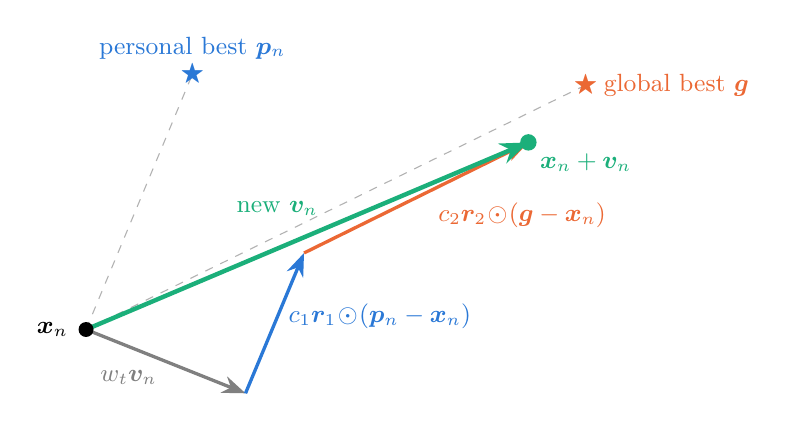
\begin{tikzpicture}[>=Stealth, scale=1.35, every node/.style={font=\small}]
  \coordinate (x) at (0,0);
  \coordinate (p) at (1.0,2.4);
  \coordinate (g) at (4.7,2.3);
  \coordinate (a) at (1.5,-0.6);
  \coordinate (ab) at ($(a)+(0.55,1.32)$);
  \coordinate (abc) at ($(ab)+(2.11,1.04)$);
  \draw[gray!60, dashed] (x) -- (p);
  \draw[gray!60, dashed] (x) -- (g);
  \draw[->, very thick, gray] (x) -- node[below left=-1pt]{$w_t\bm v_n$} (a);
  \draw[->, very thick, pdblue] (a) -- node[right, pos=0.55]{$c_1\bm r_1\!\odot\!(\bm p_n-\bm x_n)$} (ab);
  \draw[->, very thick, accent] (ab) -- node[below right=0pt, pos=0.55]{$c_2\bm r_2\!\odot\!(\bm g-\bm x_n)$} (abc);
  \draw[->, ultra thick, psogreen] (x) -- node[above left=0pt, pos=0.55]{new $\bm v_n$} (abc);
  \fill (x) circle (2pt) node[left=3pt]{$\bm x_n$};
  \fill[psogreen] (abc) circle (2.2pt) node[below right=1pt]{$\bm x_n + \bm v_n$};
  \node[pdblue] at (p) {$\bigstar$};
  \node[pdblue, above=2pt] at (p) {personal best $\bm p_n$};
  \node[accent] at (g) {$\bigstar$};
  \node[accent, right=3pt] at (g) {global best $\bm g$};
\end{tikzpicture}
\caption{One PSO step. The new velocity is the sum of the damped previous velocity (grey), a random pull
towards the particle's own best (blue) and a random pull towards the swarm's best (orange). The random
factors are drawn as scalars for clarity; in the algorithm they differ per dimension.}
\label{fig:velocity}
\end{figure}

\subsection{Inertia weight: from exploration to exploitation}

The inertia weight $w$ was added by Shi and Eberhart \cite{shi1998}. A large $w$ makes particles keep their
speed and roam widely (exploration). A small $w$ makes them slow down and search finely around the best
points found (exploitation). The implementation decreases $w$ linearly over the run,
\begin{equation}
w_t = w_{\mathrm{start}} - \left(w_{\mathrm{start}} - w_{\mathrm{end}}\right)\frac{t}{T - 1},
\qquad t = 0, \ldots, T-1,
\label{eq:inertia}
\end{equation}
from $w_{\mathrm{start}} = 0.9$ to $w_{\mathrm{end}} = 0.4$ over $T = 60$ iterations, the schedule
recommended in \cite{shi1998}. Early iterations explore; late iterations refine.

\subsection{Acceleration coefficients and stability of the swarm}

The coefficients $c_1$ (cognitive) and $c_2$ (social) set the strength of the two attractions. Here
$c_1 = c_2 = 1.6$, so a particle trusts its own experience and the swarm's knowledge equally. If
$c_2 \gg c_1$, the swarm rushes towards the current global best and risks converging prematurely. If
$c_1 \gg c_2$, the particles behave like independent local searchers.

Not every combination of $w$, $c_1$, $c_2$ makes the swarm converge. Clerc and Kennedy \cite{clerc2002}
analysed the particle dynamics as a second-order linear system and showed how the parameters decide
between oscillation, convergence and ``explosion''. As a safeguard, the code rescales the two coefficients,
keeping their ratio, whenever $c_1 + c_2 > 4$; with $c_1 + c_2 = 3.2$ this safeguard is inactive. A more
detailed result by Poli \cite{poli2009} gives the region where the position of a particle has bounded mean
and variance (order-2 stability) during stagnation:
\begin{equation}
c_1 + c_2 < \frac{24\,(1 - w^2)}{7 - 5w}.
\label{eq:poli}
\end{equation}
For $w = 0.9$ the bound is $1.82$, and for $w = 0.4$ it is $4.03$. With $c_1 + c_2 = 3.2$ the swarm is
therefore \emph{outside} this region at the start of the run and \emph{inside} it once $w$ drops below
$0.755$, that is from iteration $18$ onwards. The first third of the run is deliberately explosive, wide
exploration held in check by velocity clamping and the walls, and the rest of the run is convergent.
Section~\ref{sec:behaviour} shows this transition in the measured swarm diversity.

\subsection{Velocity clamping}

Each velocity component is limited to a fraction of the search range \cite{eberhart2000}:
\begin{equation}
\bm v_n \leftarrow \clip\!\left(\bm v_n,\; -\bm v_{\max},\; \bm v_{\max}\right),\qquad
\bm v_{\max} = 0.2\,(\bm u - \bm l).
\end{equation}
No gain can change by more than $20\,\%$ of its range in one iteration. Clamping prevents the large
velocities of the explosive phase from throwing particles out of the box at every step.

\subsection{Boundary handling: reflective walls}

A particle that leaves the box after \eqref{eq:position} is mirrored back inside, and the offending
velocity component is reversed and halved:
\begin{equation}
x_{n,j} \leftarrow
\begin{cases}
2l_j - x_{n,j}, & x_{n,j} < l_j,\\
2u_j - x_{n,j}, & x_{n,j} > u_j,
\end{cases}
\qquad v_{n,j} \leftarrow -\tfrac12\,v_{n,j}\quad\text{(only if the wall was hit)},
\end{equation}
followed by a final clip for safety. Simply clipping positions would make particles pile up on the
boundary. Reflection keeps them inside and moving.

\subsection{Neighbourhood topology}

This implementation uses the \emph{global-best} (star) topology: every particle is attracted to the single
best position of the whole swarm. It spreads information fastest and converges quickly, which suits a
budget of only $60$ iterations. The alternative, a \emph{local-best} topology in which each particle only
knows the best of a few neighbours, converges more slowly but is less prone to premature convergence.

\subsection{The algorithm}

\begin{algorithm}[H]
\caption{Global-best PSO with decreasing inertia, as implemented in \code{src/optimizers/pso.py}}
\label{alg:pso}
\begin{algorithmic}[1]
\State Draw positions $\bm x_n \sim \mathcal U(\bm l, \bm u)$, $n = 1,\ldots,N$; overwrite the first ones with the seed designs $\bm x_0$
\State Draw velocities $\bm v_n \sim \mathcal U(-\bm v_{\max}, \bm v_{\max})$
\State Evaluate $f_n = F(\bm x_n)$ for the whole swarm; set $\bm p_n \gets \bm x_n$ and $\bm g \gets \bm p_{\arg\min f_n}$
\For{$t = 0, \ldots, T-1$}
  \State $w_t \gets w_{\mathrm{start}} - (w_{\mathrm{start}} - w_{\mathrm{end}})\,t/(T-1)$
  \State Draw $\bm r_1, \bm r_2$; update every velocity with \eqref{eq:velocity}; clamp it to $\pm\bm v_{\max}$
  \State Move every particle with \eqref{eq:position}; reflect at the walls
  \State Evaluate $f_n = F(\bm x_n)$ for the whole swarm in one call
  \State \textbf{for all} $n$ with $f_n < F(\bm p_n)$: $\bm p_n \gets \bm x_n$
  \State \textbf{if} $\min_n F(\bm p_n) < F(\bm g)$: $\bm g \gets \bm p_{\arg\min_n F(\bm p_n)}$
  \State Record $F(\bm g)$, the mean of $f_n$ and a snapshot of the swarm
\EndFor
\State \Return $\bm g$, $F(\bm g)$
\end{algorithmic}
\end{algorithm}

The global best can only improve, so the returned solution is never worse than the best initial particle.
A run costs $N + TN = 30 + 60 \times 30 = 1830$ cost evaluations.

\begin{table}[H]
\centering
\small
\begin{tabularx}{\linewidth}{@{}l c X@{}}
\toprule
\textbf{Parameter} (YAML key) & \textbf{Value} & \textbf{Role}\\
\midrule
Swarm size $N$ (\code{swarm_size}) & 30 & Number of particles: more particles explore more, at a proportional cost.\\
Iterations $T$ (\code{iterations}) & 60 & Number of updates of the swarm.\\
Initial inertia $w_{\mathrm{start}}$ (\code{w_start}) & 0.9 & Exploration at the start.\\
Final inertia $w_{\mathrm{end}}$ (\code{w_end}) & 0.4 & Exploitation at the end.\\
Cognitive coefficient $c_1$ (\code{c1}) & 1.6 & Pull towards the particle's own best.\\
Social coefficient $c_2$ (\code{c2}) & 1.6 & Pull towards the swarm's best.\\
Velocity clamp (\code{v_max_frac}) & 0.2 & Maximum step per iteration, as a fraction of each gain's range.\\
Random seed (\code{--seed}) & 0 & Makes a run reproducible.\\
\bottomrule
\end{tabularx}
\caption{PSO parameters (\code{optimization.pso} in \code{config/robot_params.yaml}).}
\label{tab:psoparams}
\end{table}

\subsection{Implementation}

The complete optimiser is the following function from \file{src/optimizers/pso.py}:
\begin{lstlisting}[style=py]
import numpy as np

from . import OptimizationResult


def pso(cost_fn, lb, ub, swarm_size=30, iterations=60, w_start=0.9, w_end=0.4, c1=1.6, c2=1.6,
        v_max_frac=0.2, seed=None, x0=None, callback=None, **_):
    rng = np.random.default_rng(seed)
    lb, ub = np.asarray(lb, float), np.asarray(ub, float)
    span = ub - lb
    if c1 + c2 > 4.0:
        c1, c2 = 4.0 * c1 / (c1 + c2), 4.0 * c2 / (c1 + c2)
    v_max = v_max_frac * span

    x = lb + rng.random((swarm_size, lb.size)) * span
    if x0 is not None:
        x0 = np.atleast_2d(x0)
        x[: len(x0)] = np.clip(x0, lb, ub)
    v = rng.uniform(-v_max, v_max, x.shape)
    f = cost_fn(x)
    p_best, p_cost = x.copy(), f.copy()
    g = np.argmin(p_cost)
    g_best, g_cost = p_best[g].copy(), p_cost[g]
    res = OptimizationResult(g_best, g_cost, [g_cost], [float(np.mean(f))], [x.copy()],
                             swarm_size, "PSO")

    for it in range(iterations):
        w = w_start - (w_start - w_end) * it / max(1, iterations - 1)
        r1, r2 = rng.random(x.shape), rng.random(x.shape)
        v = w * v + c1 * r1 * (p_best - x) + c2 * r2 * (g_best - x)
        v = np.clip(v, -v_max, v_max)
        x = x + v
        low, high = x < lb, x > ub
        x = np.where(low, 2 * lb - x, np.where(high, 2 * ub - x, x))
        v = np.where(low | high, -0.5 * v, v)
        x = np.clip(x, lb, ub)

        f = cost_fn(x)
        improved = f < p_cost
        p_best[improved], p_cost[improved] = x[improved], f[improved]
        g = np.argmin(p_cost)
        if p_cost[g] < g_cost:
            g_best, g_cost = p_best[g].copy(), p_cost[g]

        res.best_history.append(float(g_cost))
        res.mean_history.append(float(np.mean(f)))
        res.positions.append(x.copy())
        res.n_evals += swarm_size
        if callback:
            callback(it, g_best, g_cost)

    res.best_x, res.best_cost = g_best, float(g_cost)
    return res
\end{lstlisting}

\begin{table}[H]
\centering
\small
\begin{tabularx}{\linewidth}{@{}l X@{}}
\toprule
\textbf{Lines} & \textbf{What they do}\\
\midrule
6--7 & Signature: the cost function, the bounds, the parameters of Table~\ref{tab:psoparams}, a seed, optional seed designs \code{x0} and an optional progress \code{callback}.\\
8 & Seeded random generator: identical seeds give identical runs.\\
11--12 & Coefficient safeguard: rescale $c_1$, $c_2$ if their sum exceeds 4.\\
13 & Velocity limit $\bm v_{\max} = 0.2(\bm u - \bm l)$.\\
15--19 & Initial swarm: uniform positions, known designs injected into the first rows, uniform velocities.\\
20--23 & Evaluate the whole swarm at once; initialise personal and global bests.\\
24--25 & Result object storing the best cost, mean cost and swarm snapshot of every iteration.\\
28 & Inertia schedule \eqref{eq:inertia}.\\
29--30 & Velocity update \eqref{eq:velocity}, vectorised over all particles and dimensions.\\
31--32 & Velocity clamp and position update \eqref{eq:position}.\\
33--36 & Reflective walls with velocity reversal and halving, then a safety clip.\\
38--43 & Evaluate the swarm; update the personal bests that improved and, if beaten, the global best.\\
45--50 & Record the history and report progress.\\
\bottomrule
\end{tabularx}
\caption{Line-by-line map of the implementation.}
\end{table}

The optimiser knows nothing about robots or PID controllers: it only sees a vector-valued cost function and
a box. Everything specific to the tuning problem lives in the cost function, described next.

%=====================================================================================================
\section{Applying PSO to PID tuning}
\label{sec:application}
%=====================================================================================================

\subsection{What a particle is}

A particle is a complete set of controller gains for the three joints, stacked joint by joint:
\begin{equation}
\bm x = \left[K_{p1}, K_{i1}, K_{d1},\; K_{p2}, K_{i2}, K_{d2},\; K_{p3}, K_{i3}, K_{d3}\right] \in \mathbb{R}^9.
\end{equation}
Every joint shares the same search box, in Table~\ref{tab:bounds}. The swarm therefore moves in a
nine-dimensional space, and every point of that space is a full controller design.

\begin{table}[H]
\centering
\begin{tabular}{lccc}
\toprule
Loop & $K_p$ & $K_i$ & $K_d$\\
\midrule
Joint position (main case) & $[0.1,\ 8]$ & $[0,\ 8]$ & $[0,\ 0.4]$\\
Joint velocity (task-space controller, Section~\ref{sec:taskspace}) & $[0.001,\ 0.5]$ & $[0,\ 10]$ & $[0,\ 0.005]$\\
\bottomrule
\end{tabular}
\caption{Search bounds per joint (\code{optimization.bounds}).}
\label{tab:bounds}
\end{table}

\subsection{How a particle is evaluated}

Figure~\ref{fig:evaluate} summarises the evaluation. The particle is split into the gains of the three
joints. Each joint's closed loop is simulated for a $0.3\,\mathrm{rad}$ ($17.2^\circ$) step, once with a
local $1\,\mathrm{kHz}$ loop and once with the feedback delayed by one UDP period ($20\,\mathrm{ms}$). Each
response is reduced to performance metrics, the stability margins are computed from the frequency response,
and everything is combined into one number. The following subsections describe each block.

\begin{figure}[H]
\centering
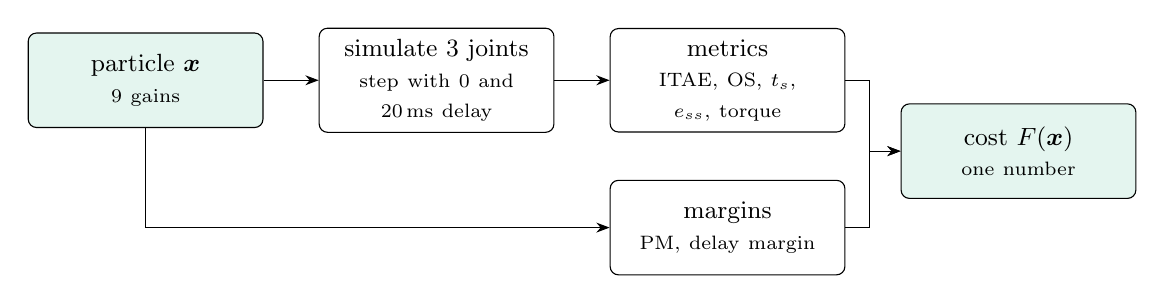
\begin{tikzpicture}[>=Stealth, node distance=6mm and 7mm,
  box/.style={draw, rounded corners=3pt, align=center, font=\small, minimum height=12mm, inner sep=4pt, fill=white, text width=27mm},
  hl/.style={box, fill=psogreen!12}]
  \node[hl] (x) {particle $\bm x$\\\scriptsize 9 gains};
  \node[box, right=of x] (sim) {simulate 3 joints\\\scriptsize step with 0 and 20\,ms delay};
  \node[box, right=of sim] (met) {metrics\\\scriptsize ITAE, OS, $t_s$, $e_{ss}$, torque};
  \node[box, below=of met] (mar) {margins\\\scriptsize PM, delay margin};
  \node[hl, right=of met, yshift=-9mm] (F) {cost $F(\bm x)$\\\scriptsize one number};
  \draw[->] (x) -- (sim);
  \draw[->] (sim) -- (met);
  \draw[->] (x.south) |- (mar);
  \draw[->] (met.east) -- ++(3mm,0) |- (F.west);
  \draw[->] (mar.east) -- ++(3mm,0) |- (F.west);
\end{tikzpicture}
\caption{Evaluating one particle. In practice the whole swarm ($30$ particles $\times$ $3$ joints) is
evaluated simultaneously.}
\label{fig:evaluate}
\end{figure}

\subsection{Plant model}

Each actuated joint is modelled as an independent rotating inertia with viscous damping and a disturbance
torque:
\begin{equation}
J_i\,\ddot q_i + B_i\,\dot q_i + b_i + c_i\tanh\!\left(\frac{\dot q_i}{v_s}\right) = \tau_i,
\qquad |\tau_i| \le \tau_{\max,i}.
\label{eq:plant}
\end{equation}
The constant $b_i$ represents gravity and static load. The $\tanh$ term is a smooth approximation of
Coulomb friction ($v_s = 0.01\,\mathrm{rad/s}$). The bias values were chosen so that the thesis PD gains
reproduce the documented $3$--$8^\circ$ steady-state error. Without disturbance the plant is
$H_i(s) = 1/\left(s\,(J_i s + B_i)\right)$.

\begin{table}[H]
\centering
\begin{tabular}{lcccccc}
\toprule
Joint & $J_i$ [kg\,m$^2$] & $B_i$ [N\,m\,s/rad] & $b_i$ [N\,m] & $c_i$ [N\,m] & $\tau_{\max,i}$ [N\,m] & $\tau_{\mathrm{cont},i}$ [N\,m]\\
\midrule
1 (base)     & 0.0031 & 0.0089 & 0.100 & 0.010 & 0.865 & 0.231\\
2 (shoulder) & 0.0022 & 0.0170 & 0.200 & 0.015 & 0.865 & 0.231\\
3 (elbow)    & 0.0009 & 0.0058 & 0.050 & 0.008 & 0.432 & 0.115\\
\bottomrule
\end{tabular}
\caption{Joint parameters. Torque limits: $3.3\,\mathrm{N}$ peak and $0.88\,\mathrm{N}$ continuous tip force
times the lever arm ($0.262\,\mathrm{m}$ for joints 1--2, $0.131\,\mathrm{m}$ for joint 3).}
\label{tab:plant}
\end{table}

The controller runs at $T_s = 1\,\mathrm{ms}$. Between samples the torque is held constant and
\eqref{eq:plant} is integrated with fourth-order Runge--Kutta. A feedback delay $\tau_d$ is modelled by
giving the controller the measurement taken $\tau_d/T_s$ samples earlier (Figure~\ref{fig:loop}).

\begin{figure}[H]
\centering
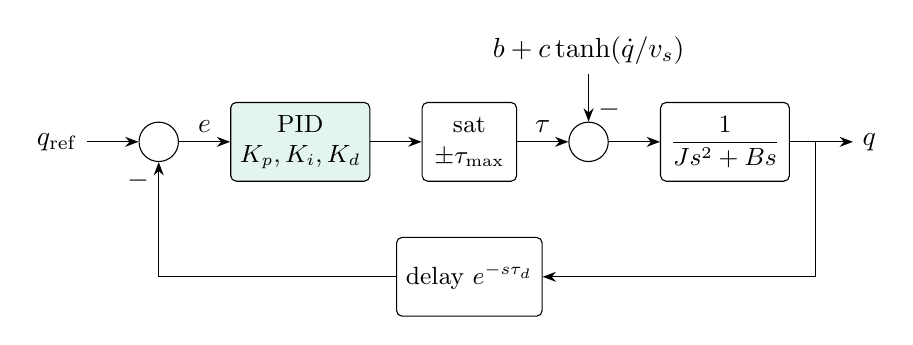
\begin{tikzpicture}[>=Stealth, node distance=5mm and 6.5mm,
  blk/.style={draw, rounded corners=2pt, minimum height=10mm, minimum width=12mm, align=center, font=\small, fill=white},
  sum/.style={draw, circle, inner sep=0pt, minimum size=5mm}]
  \node (r) {$q_{\mathrm{ref}}$};
  \node[sum, right=of r] (s1) {};
  \node[blk, right=of s1, fill=psogreen!12] (pid) {PID\\$K_p, K_i, K_d$};
  \node[blk, right=of pid] (sat) {sat\\$\pm\tau_{\max}$};
  \node[sum, right=of sat] (s2) {};
  \node[blk, right=of s2] (pl) {$\dfrac{1}{J s^2 + B s}$};
  \node[right=8mm of pl] (q) {$q$};
  \node[blk, below=7mm of sat] (del) {delay $e^{-s\tau_d}$};
  \node[above=6mm of s2] (d) {$b + c\tanh(\dot q/v_s)$};
  \draw[->] (r) -- (s1);
  \draw[->] (s1) -- node[above]{$e$} (pid);
  \draw[->] (pid) -- (sat);
  \draw[->] (sat) -- node[above]{$\tau$} (s2);
  \draw[->] (s2) -- (pl);
  \draw[->] (pl) -- coordinate[pos=0.4] (tap) (q);
  \draw[->] (tap) |- (del);
  \draw[->] (del) -| node[pos=0.92, left]{$-$} (s1);
  \draw[->] (d) -- node[pos=0.75, right]{$-$} (s2);
\end{tikzpicture}
\caption{Simulated joint loop. PSO chooses the three gains of the green block.}
\label{fig:loop}
\end{figure}

\subsection{Controller}

The discrete PID that the swarm tunes is (\code{DiscretePID} in \file{src/controllers.py})
\begin{align}
u_k^{*} &= K_p\,e_k + I_k + K_d\,\delta_k,\qquad u_k = \sat\!\left(u_k^{*}, \pm\tau_{\max}\right),\qquad e_k = r_k - y_k,\\
\delta_k &= \delta_{k-1} + \alpha\left(-\frac{y_k - y_{k-1}}{T_s} - \delta_{k-1}\right),\qquad
\alpha = \frac{T_s}{T_f + T_s},\quad T_f = \frac{1}{2\pi\cdot 100\,\mathrm{Hz}},\\
I_{k+1} &= \begin{cases} I_k, & \text{output saturated and } \sgn e_k = \sgn u_k^{*},\\ I_k + K_i T_s e_k, & \text{otherwise.}\end{cases}
\end{align}
The derivative acts on the measurement, which avoids a torque spike when the reference steps. It is
low-pass filtered at $100\,\mathrm{Hz}$ to limit noise amplification. The integrator is frozen while the
output saturates in the direction of the error, which prevents integrator wind-up. For frequency analysis
the controller is $C(s) = K_p + K_i/s + K_d s/(1 + T_f s)$.

\subsection{Performance metrics}

For a step of amplitude $A$, with $e_k = A - y_k$ and $t_k = kT_s$, \code{step_metrics} computes:
\begin{itemize}[nosep]
  \item the integral of time-weighted absolute error, $\mathrm{ITAE} = \frac{T_s}{|A|}\sum_k t_k|e_k|$,
        which penalises slow convergence and lingering offsets;
  \item the overshoot $\mathrm{OS} = \max(0, \max_k y_k/A - 1)$;
  \item the settling time $t_s$ into a $\pm2\,\%$ band (the full horizon if never reached);
  \item the steady-state error $e_{ss}$, the mean of $|e_k|/|A|$ over the last $0.1\,\mathrm{s}$;
  \item the RMS torque $\tau_{\mathrm{rms}}$;
  \item a divergence flag: non-finite output, $|y| > 5|A|$, or a sustained oscillation of more than $10\,\%$
        of $|A|$ in the last $0.3\,\mathrm{s}$.
\end{itemize}

\subsection{Stability margins}

From the open-loop response $L(j\omega) = C(j\omega)H(j\omega)e^{-j\omega T_s/2}$ (the exponential models the
average half-sample delay of sampling), \code{stability_margins} finds the gain crossover $\omega_c$ where
$|L| = 1$ and returns
\begin{equation}
\mathrm{PM} = 180^\circ + \angle L(j\omega_c),\qquad \tau_{d,\max} = \frac{\mathrm{PM}\,[\mathrm{rad}]}{\omega_c}.
\label{eq:dm}
\end{equation}
The delay margin $\tau_{d,\max}$ is the extra loop delay that would make the loop marginally stable. For the
thesis PD in the ideal case it gives exactly the thesis values ($\omega_c = 35\,\mathrm{rad/s}$,
$\mathrm{PM} = 70^\circ$, $\tau_{d,\max} = 34.9\,\mathrm{ms}$). With the derivative filter and sampling
delay included, the thesis PD has $\tau_{d,\max} \approx 32.6\,\mathrm{ms}$.

\subsection{The fitness function}

For joint $i$ under delay $\delta$, the metrics are combined as
\begin{equation}
c_{i,\delta} =
\begin{cases}
4\,\mathrm{ITAE} + 2\,\mathrm{OS} + 1\,t_s + 10\,e_{ss} + 0.5\max\!\left(0, \dfrac{\tau_{\mathrm{rms}}}{\tau_{\mathrm{cont},i}} - 1\right), & \text{stable},\\[8pt]
1000, & \text{diverged},
\end{cases}
\end{equation}
and the fitness of a particle is
\begin{equation}
F(\bm x) = \sum_{i=1}^{3}\left[\frac{c_{i,0} + c_{i,20\,\mathrm{ms}}}{2}
+ 5\,\frac{\max(0,\; 45^\circ - \mathrm{PM}_i)}{45^\circ}
+ 5\,\frac{\max(0,\; 30\,\mathrm{ms} - \tau_{d,\max,i})}{30\,\mathrm{ms}}\right].
\label{eq:cost}
\end{equation}
The design choices behind this function:
\begin{itemize}
  \item \textbf{Averaging over two delays} makes the swarm prefer gains that work both locally and over the
        network, instead of the fastest local response.
  \item \textbf{The fixed cost of 1000 for divergence} gives unstable particles a very bad, but finite,
        score. PSO handles this naturally: such particles are simply never chosen as personal or global
        bests.
  \item \textbf{Soft penalties} below $45^\circ$ of phase margin and $30\,\mathrm{ms}$ ($1.5$ UDP periods) of
        delay margin act as constraints without making the cost undefined.
  \item \textbf{The torque term} penalises only the RMS torque above the continuous motor rating, the part
        that would overheat the motor.
\end{itemize}
On this fitness the thesis PD design scores $F = 18.54$: almost all of it comes from its steady-state error
and from never settling into the $\pm2\,\%$ band.

\subsection{Seeding the swarm with the thesis design}

The thesis PD gains are injected as one of the $30$ initial particles (the \code{x0} argument). Because
the global best never gets worse, this guarantees that PSO returns a design at least as good as the
thesis. The measurements in Section~\ref{sec:behaviour} show that this matters: all $29$ random initial
particles produce at least one unstable loop, so the seeded design is the only stable starting point.

\subsection{Evaluating the whole swarm at once}

The simulator and the cost function are vectorised. Gains are arrays of shape $(N, 3)$, so one time step
advances all $30 \times 3 = 90$ joint loops with a few NumPy array operations. PSO calls the cost function
once per iteration with the whole swarm. A complete run, $61$ swarm evaluations, each simulating two delay
scenarios of $1500$ RK4 steps, takes about $15$--$30\,\mathrm{s}$ on a desktop PC.

%=====================================================================================================
\section{How the swarm behaves}
\label{sec:behaviour}
%=====================================================================================================

This section looks inside the reference run (seed 0, the gains stored in
\file{results/gains_position.json}) and then repeats the run with ten seeds. Iteration $0$ denotes the
initial swarm and iteration $k$ the swarm after $k$ updates. All figures and numbers in this section were
produced by \file{docs/make_pso_figures.py}, which reruns PSO and reproduces the stored gains exactly.

\subsection{Convergence}

\begin{figure}[H]
\centering
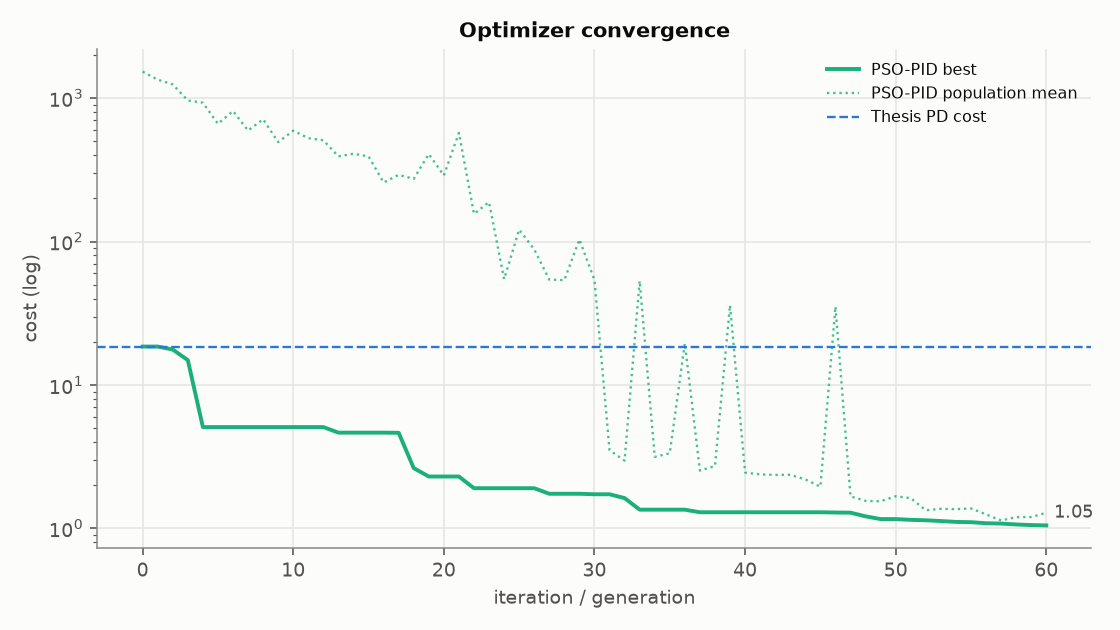
\includegraphics[width=0.8\linewidth]{pso_convergence.png}
\caption{Best cost (solid) and mean cost of the swarm (dotted) per iteration, log scale. The dashed line is
the cost of the thesis PD.}
\label{fig:conv}
\end{figure}

The best cost (Figure~\ref{fig:conv}) starts at the thesis PD value of $18.54$, because the seeded design
is the best initial particle. It drops to $5.09$ within five iterations, which is already almost four times
better than the thesis, then improves in steps to $1.05$ after $60$ iterations, a $17.7$-fold
improvement. The mean cost of the swarm starts above $1500$, because almost every random particle is
unstable and costs $1000$ per diverged loop. It falls to about $2.5$ at iteration $40$ and $1.3$ at the
end, once the whole swarm sits in the stable region. Its late spikes (iterations 39 and 46) are single
particles overshooting into an unstable region: one diverged loop adds about $1000/30 \approx 33$ to the
mean.

\subsection{From exploration to exploitation}

\begin{figure}[H]
\centering
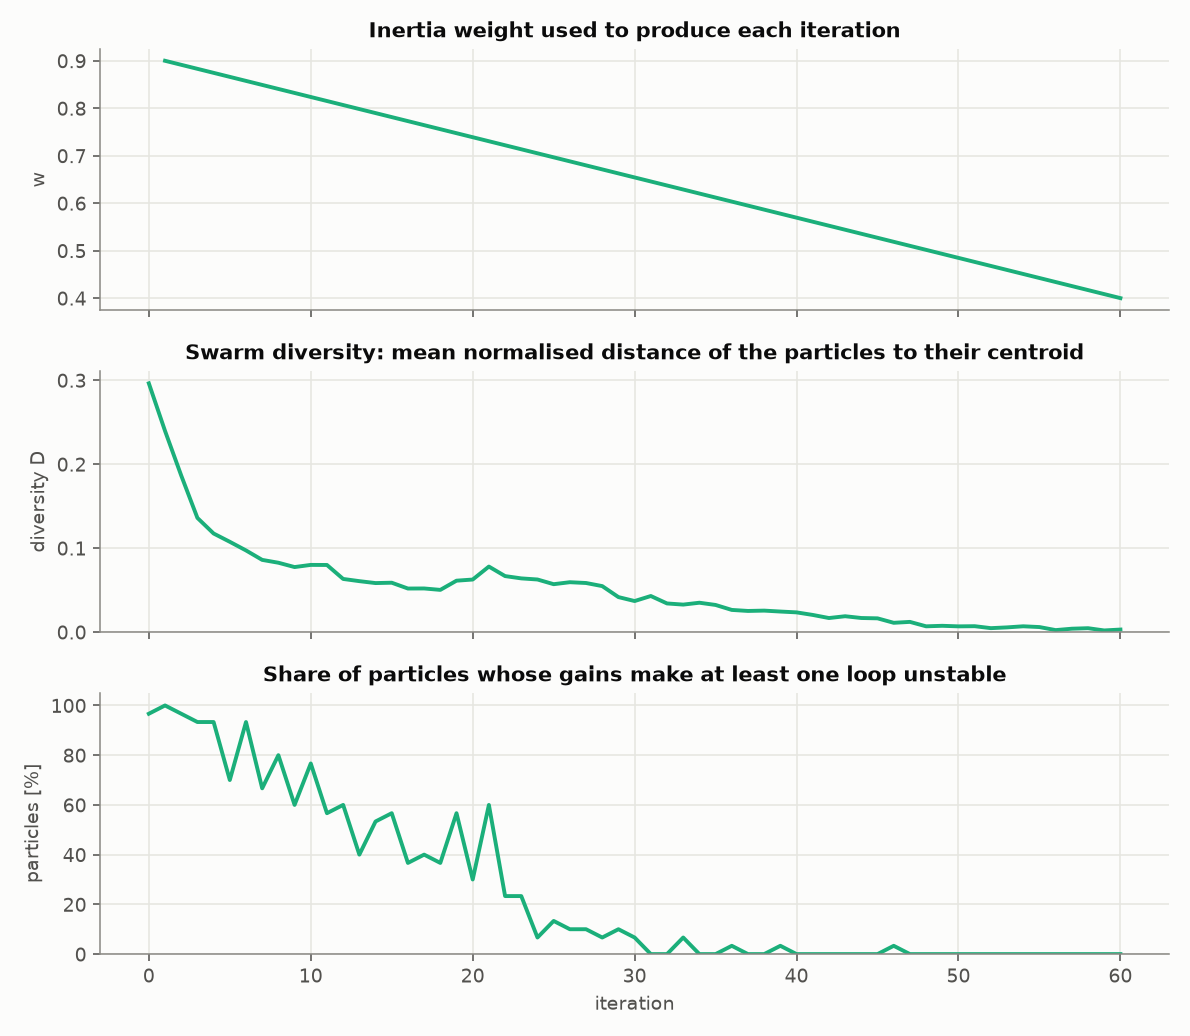
\includegraphics[width=0.8\linewidth]{pso_swarm_dynamics.png}
\caption{Inside the swarm. Top: inertia weight. Middle: diversity $D$, the mean distance of the particles to
their centroid, with every gain normalised to its range ($0$ means all particles coincide). Bottom: share of
particles whose gains make at least one of the six simulated loops unstable.}
\label{fig:dynamics}
\end{figure}

\begin{table}[H]
\centering
\begin{tabular}{rrrrr}
\toprule
Iteration & Best cost & Mean cost & Diversity $D$ & Unstable particles\\
\midrule
0  & 18.540 & 1531.6 & 0.296 & 96.7\,\%\\
5  & 5.089  & 662.3  & 0.108 & 70.0\,\%\\
10 & 5.089  & 593.3  & 0.080 & 76.7\,\%\\
20 & 2.302  & 289.2  & 0.063 & 30.0\,\%\\
30 & 1.731  & 53.9   & 0.037 & 6.7\,\%\\
40 & 1.297  & 2.45   & 0.023 & 0\,\%\\
50 & 1.162  & 1.68   & 0.007 & 0\,\%\\
60 & 1.050  & 1.28   & 0.003 & 0\,\%\\
\bottomrule
\end{tabular}
\caption{Swarm statistics of the reference run.}
\label{tab:dynamics}
\end{table}

Figure~\ref{fig:dynamics} and Table~\ref{tab:dynamics} show the two phases of a PSO run:
\begin{itemize}
  \item \textbf{Exploration (iterations 0--20).} The swarm contracts quickly from its random start
        ($D = 0.30$ to $0.11$ in five iterations) as particles are pulled towards the seeded design, but it
        keeps a moderate spread ($D \approx 0.06$--$0.08$), and most particles remain unstable. In this phase
        the parameters lie outside the stability region \eqref{eq:poli}, so particles keep overshooting
        their attractors and sampling a wide area.
  \item \textbf{Exploitation (from about iteration 20).} Once $w$ has dropped below $0.755$ (iteration
        18), the dynamics become convergent. The share of unstable particles falls from $60\,\%$ at
        iteration 21 to $23\,\%$ at iteration 22. From iteration 31 the swarm is entirely stable, apart from
        single particles straying out at iterations 33, 36, 39 and 46. The diversity decays steadily to
        $0.003$: at the end all particles nearly coincide and refine the same design.
\end{itemize}
The observed transition agrees with the stability analysis of Section~\ref{sec:pso}: the inertia schedule
first lets the swarm explore and then forces it to converge.

\subsection{The swarm in the gain space}

\begin{figure}[H]
\centering
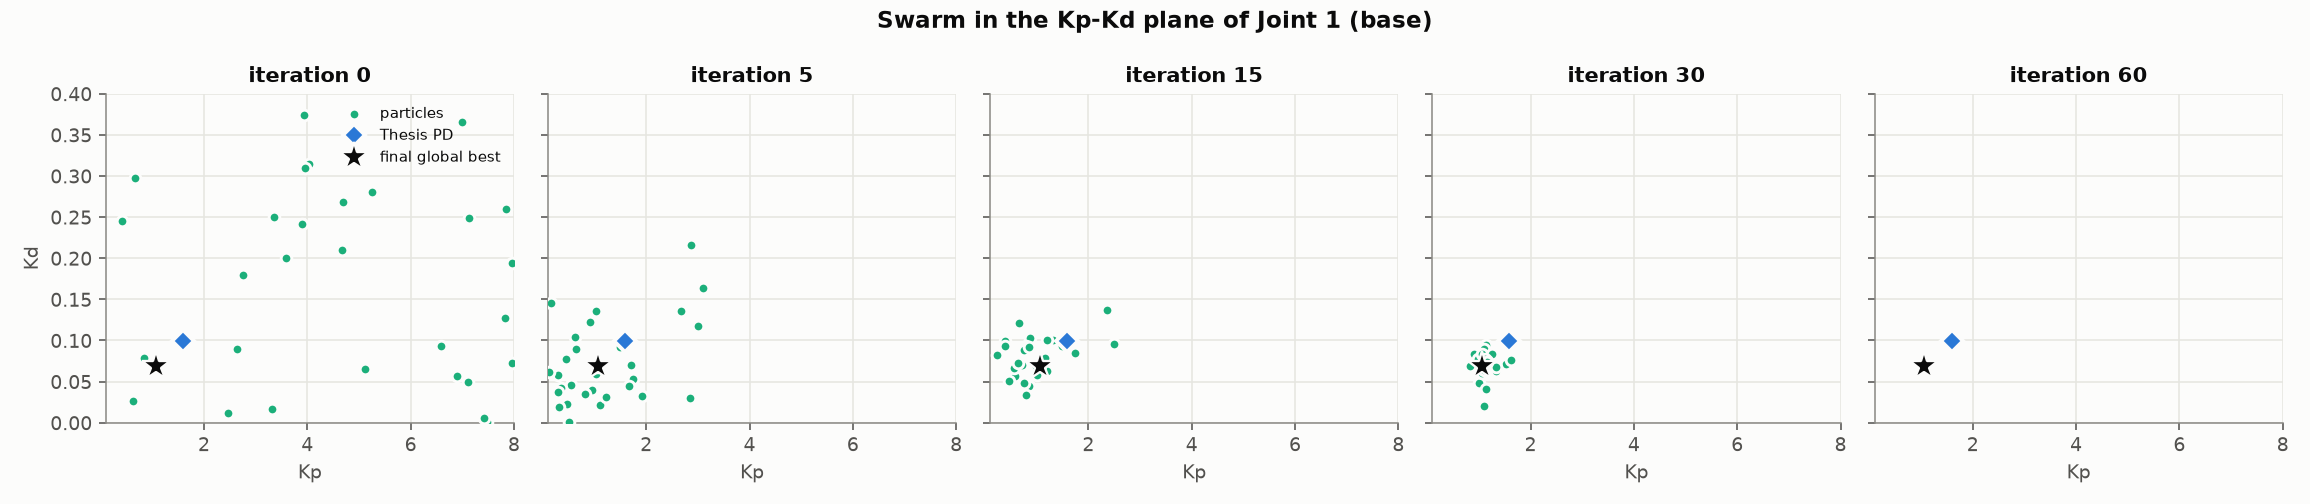
\includegraphics[width=\linewidth]{pso_swarm_kp_kd.png}\\[4pt]
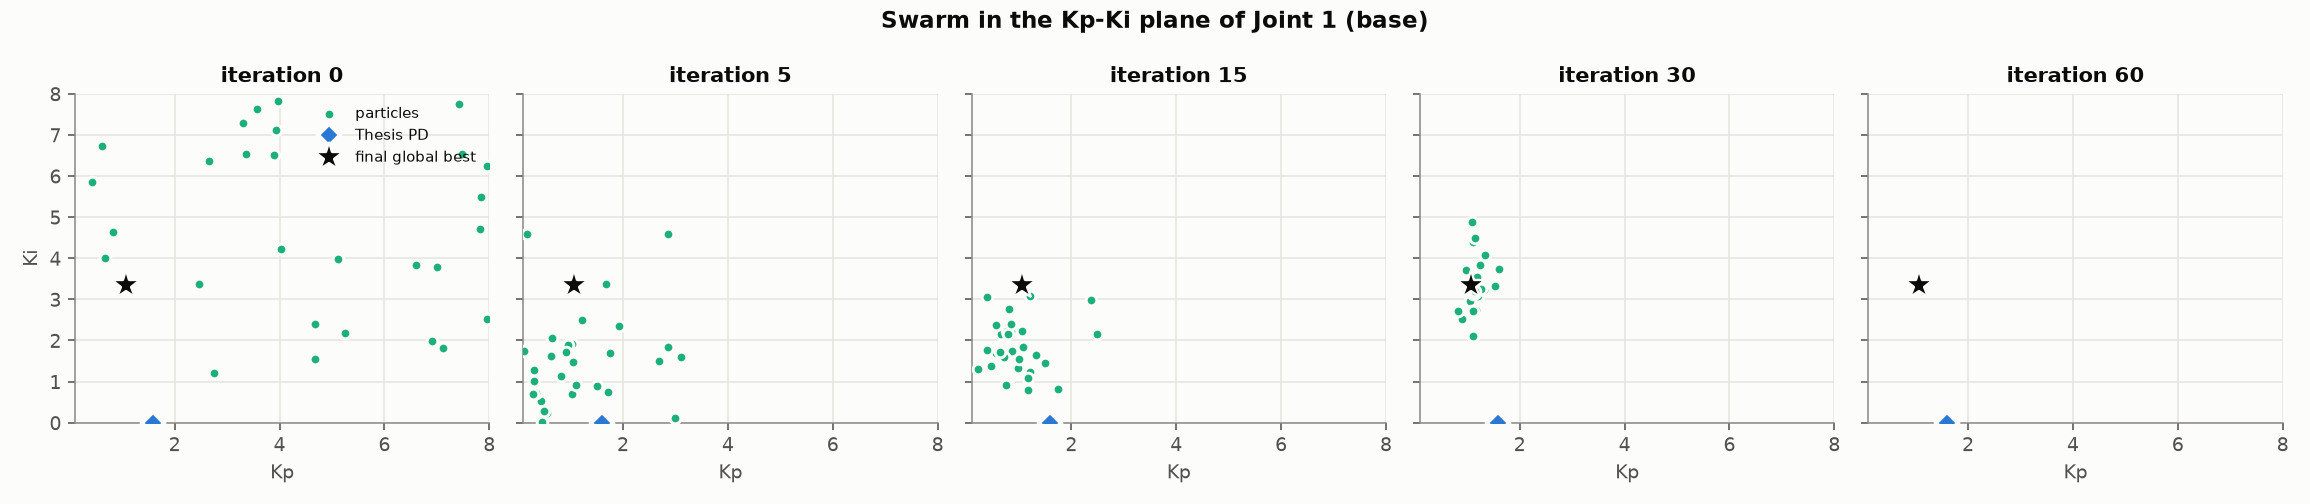
\includegraphics[width=\linewidth]{pso_swarm_kp_ki.png}
\caption{Positions of the 30 particles projected on the $K_p$--$K_d$ plane (top) and the $K_p$--$K_i$ plane
(bottom) of joint 1, at iterations 0, 5, 15, 30 and 60. Diamond: thesis PD. Star: final global best.}
\label{fig:swarm}
\end{figure}

Figure~\ref{fig:swarm} shows the same process in two projections of the nine-dimensional space. At
iteration 0 the particles cover the box uniformly. By iteration 5 most have moved to the region
$K_p < 3$, $K_d < 0.15$, near the seeded design. By iteration 30 they form a tight cloud around
$K_p \approx 1.1$, and at iteration 60 they have collapsed onto the final design. The bottom row shows the
most important discovery of the swarm: the cloud moves \emph{up}, away from the thesis design at
$K_i = 0$, to $K_i \approx 3.4$. The swarm found by itself that integral action is needed.

\subsection{Evolution of the global best}

\begin{figure}[H]
\centering
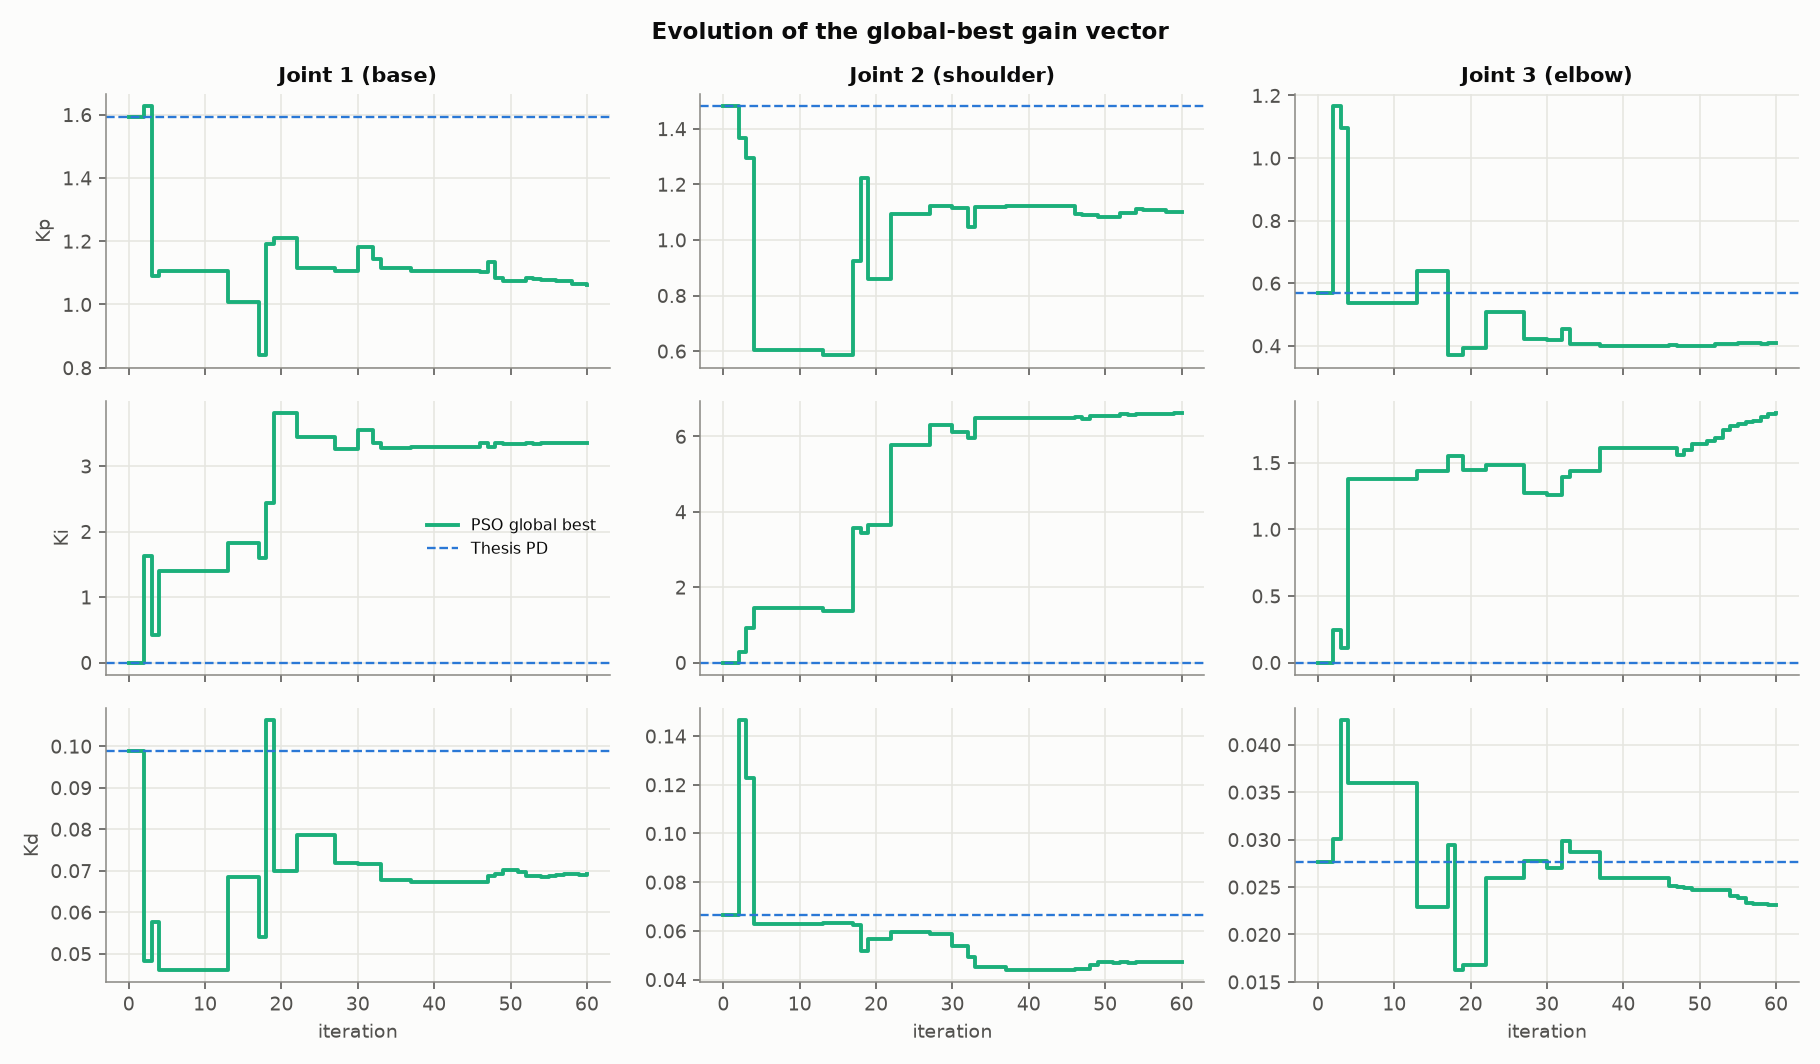
\includegraphics[width=\linewidth]{pso_gbest_evolution.png}
\caption{The nine components of the global best $\bm g$ per iteration (green) against the thesis PD gains
(dashed blue). Every change is a moment when some particle found a better design.}
\label{fig:gbest}
\end{figure}

\begin{table}[H]
\centering
\small
\begin{tabular}{r ccc ccc ccc r}
\toprule
 & \multicolumn{3}{c}{Joint 1} & \multicolumn{3}{c}{Joint 2} & \multicolumn{3}{c}{Joint 3} & \\
Iter. & $K_p$ & $K_i$ & $K_d$ & $K_p$ & $K_i$ & $K_d$ & $K_p$ & $K_i$ & $K_d$ & $F(\bm g)$\\
\midrule
0  & 1.592 & 0     & 0.0989 & 1.481 & 0     & 0.0665 & 0.568 & 0     & 0.0276 & 18.54\\
5  & 1.107 & 1.398 & 0.0462 & 0.603 & 1.450 & 0.0629 & 0.536 & 1.381 & 0.0360 & 5.09\\
20 & 1.210 & 3.805 & 0.0699 & 0.859 & 3.645 & 0.0568 & 0.392 & 1.443 & 0.0168 & 2.30\\
30 & 1.182 & 3.543 & 0.0716 & 1.115 & 6.107 & 0.0539 & 0.417 & 1.255 & 0.0270 & 1.73\\
40 & 1.106 & 3.298 & 0.0672 & 1.120 & 6.474 & 0.0441 & 0.398 & 1.607 & 0.0259 & 1.30\\
60 & 1.062 & 3.352 & 0.0691 & 1.100 & 6.612 & 0.0474 & 0.408 & 1.871 & 0.0231 & 1.05\\
\bottomrule
\end{tabular}
\caption{The global best at selected iterations.}
\label{tab:gbest}
\end{table}

Figure~\ref{fig:gbest} and Table~\ref{tab:gbest} show how the solution was built. In the first five
iterations the swarm introduced integral gains of about $1.4$ on every joint and lowered the proportional
gains, which removed most of the steady-state error and cut the cost from $18.5$ to $5.1$. Between
iterations 17 and 30 the integral gains grew further, especially on the shoulder (joint 2), which carries the
largest gravity bias ($0.2\,\mathrm{N\,m}$) and ends with the largest $K_i = 6.6$. The last 30 iterations
only fine-tune the values, in agreement with the low diversity of that phase.

\subsection{Reproducibility over random seeds}

PSO is stochastic, so one run is not enough to judge it. The tuning was repeated with seeds 0 to 9 and
otherwise identical settings.

\begin{figure}[H]
\centering
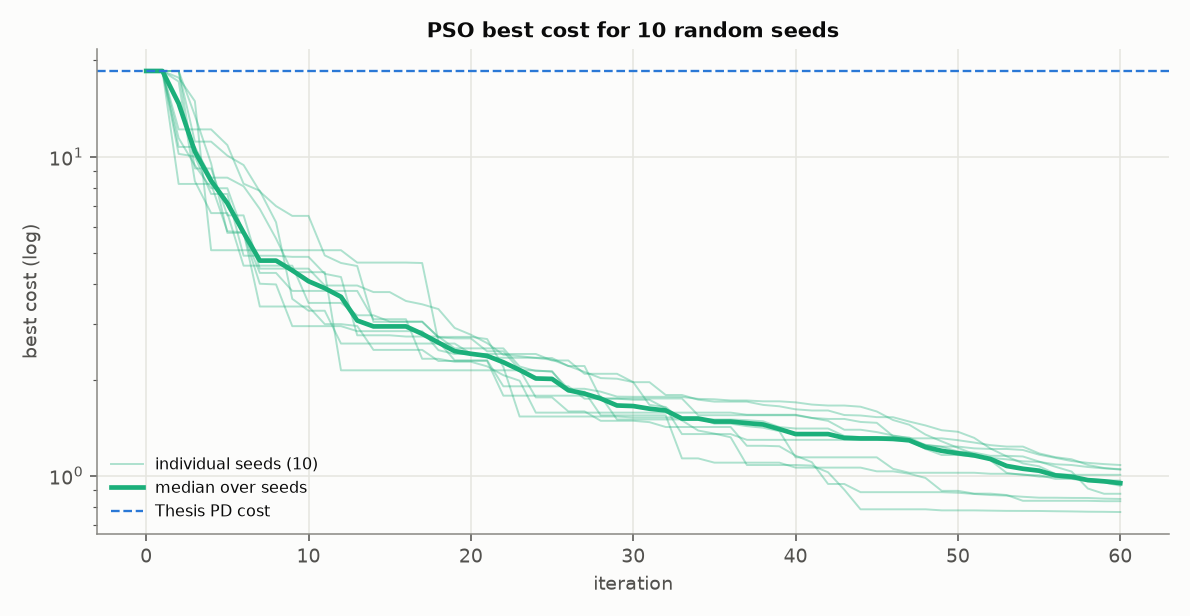
\includegraphics[width=0.8\linewidth]{pso_seeds.png}
\caption{Best cost per iteration for ten seeds (thin lines) and their median (thick line).}
\label{fig:seeds}
\end{figure}

\begin{table}[H]
\centering
\small
\begin{tabular}{rcccc}
\toprule
Seed & Final cost $F$ & Min.\ PM [$^\circ$] & Min.\ delay margin [ms] & First unstable delay [ms]\\
\midrule
0 (reference) & 1.050 & 55.6 & 38.1 & 42.5\\
1 & 1.007 & 63.6 & 32.3 & 32.5\\
2 & \textbf{0.770} & 55.6 & 31.8 & 35.0\\
3 & 0.847 & 60.8 & 32.4 & 35.0\\
4 & 0.879 & 58.7 & 30.3 & 30.0\\
5 & 0.833 & 53.9 & 31.3 & 32.5\\
6 & 0.931 & 61.1 & 31.8 & 35.0\\
7 & 1.081 & 57.8 & 33.5 & 35.0\\
8 & 1.045 & 60.5 & 30.0 & 32.5\\
9 & 0.966 & 46.6 & 30.1 & 30.0\\
\midrule
mean $\pm$ std & $0.941 \pm 0.106$ & & & \\
\bottomrule
\end{tabular}
\caption{Ten independent PSO runs. The smallest PM and delay margin are taken over the three joints. The
first unstable delay comes from a simulated sweep in steps of $2.5\,\mathrm{ms}$.}
\label{tab:seeds}
\end{table}

The seed study (Figure~\ref{fig:seeds}, Table~\ref{tab:seeds}) leads to four conclusions:
\begin{enumerate}
  \item \textbf{PSO is reliable on this problem.} All ten runs end between $0.77$ and $1.08$, that is
        $17$--$24$ times better than the thesis design, and all curves follow the same course.
  \item \textbf{The reference run is not the best one.} Seed 0 ends at $1.05$, above the median of
        $0.95$. Running PSO a few times and keeping the best result is cheap and worthwhile.
  \item \textbf{The gains differ between runs, the structure does not.} Every run uses substantial
        integral action on every joint ($K_i$ between $3.4$ and $4.6$ on joint 1, $4.5$ and $8.0$ on joint 2,
        $1.8$ and $2.6$ on joint 3), while $K_p$ and $K_d$ vary more. The cost landscape has a broad valley
        of nearly equivalent designs.
  \item \textbf{PSO satisfies the delay-margin constraint, but does not exceed it on purpose.} In nine runs
        out of ten the smallest delay margin lies between $30.0$ and $33.5\,\mathrm{ms}$, just above the
        $30\,\mathrm{ms}$ floor of \eqref{eq:cost}. The swarm trades any additional margin for a lower cost,
        as the cost function asks. The $42.5\,\mathrm{ms}$ of delay tolerance of the reference run is
        therefore a favourable outcome, not a guaranteed property. If more delay tolerance is required, the
        floor (\code{dm_min}) must be raised.
\end{enumerate}

%=====================================================================================================
\section{Performance of the PSO-tuned controller}
\label{sec:results}
%=====================================================================================================

This section evaluates the reference design (seed 0) against the two thesis baselines. The numbers come
from \file{results/summary.md}; the figures were regenerated without other optimisers by
\file{docs/make_pso_figures.py}.

\subsection{Gains and stability margins}

\begin{table}[H]
\centering
\begin{tabular}{llrrrrrr}
\toprule
Controller & Joint & $K_p$ & $K_i$ & $K_d$ & PM [$^\circ$] & $\omega_c$ [rad/s] & $\tau_{d,\max}$ [ms]\\
\midrule
Thesis PD & 1 & 1.5920 & 0 & 0.0989 & 66.6 & 35 & 32.6\\
          & 2 & 1.4810 & 0 & 0.0665 & 66.9 & 36 & 32.7\\
          & 3 & 0.5678 & 0 & 0.0276 & 66.8 & 35 & 32.7\\
\midrule
QUARC PID & 1 & 2.7262 & 1.2000 & 0.0808 & 48.4 & 36 & 23.3\\
\midrule
\textbf{PSO-PID} & 1 & 1.0621 & 3.3516 & 0.0691 & 60.4 & 25.0 & 42.2\\
                 & 2 & 1.1000 & 6.6117 & 0.0474 & 55.6 & 25.4 & 38.1\\
                 & 3 & 0.4078 & 1.8709 & 0.0231 & 65.1 & 28.0 & 40.6\\
\bottomrule
\end{tabular}
\caption{Gains and stability margins (with the $100\,\mathrm{Hz}$ derivative filter and the half-sample
delay).}
\label{tab:gains}
\end{table}

Compared with the thesis PD, PSO lowered $K_p$ and $K_d$ and added integral action. The lower gains move the
crossover from $35$ to $25$--$28\,\mathrm{rad/s}$. By \eqref{eq:dm} this raises the delay margin even though
the phase margin drops slightly: on joint 1, $60.4^\circ = 1.054\,\mathrm{rad}$ and
$1.054/25.0 = 42.2\,\mathrm{ms}$. All phase margins stay well above the $45^\circ$ floor.

\subsection{Step responses}

\begin{figure}[H]
\centering
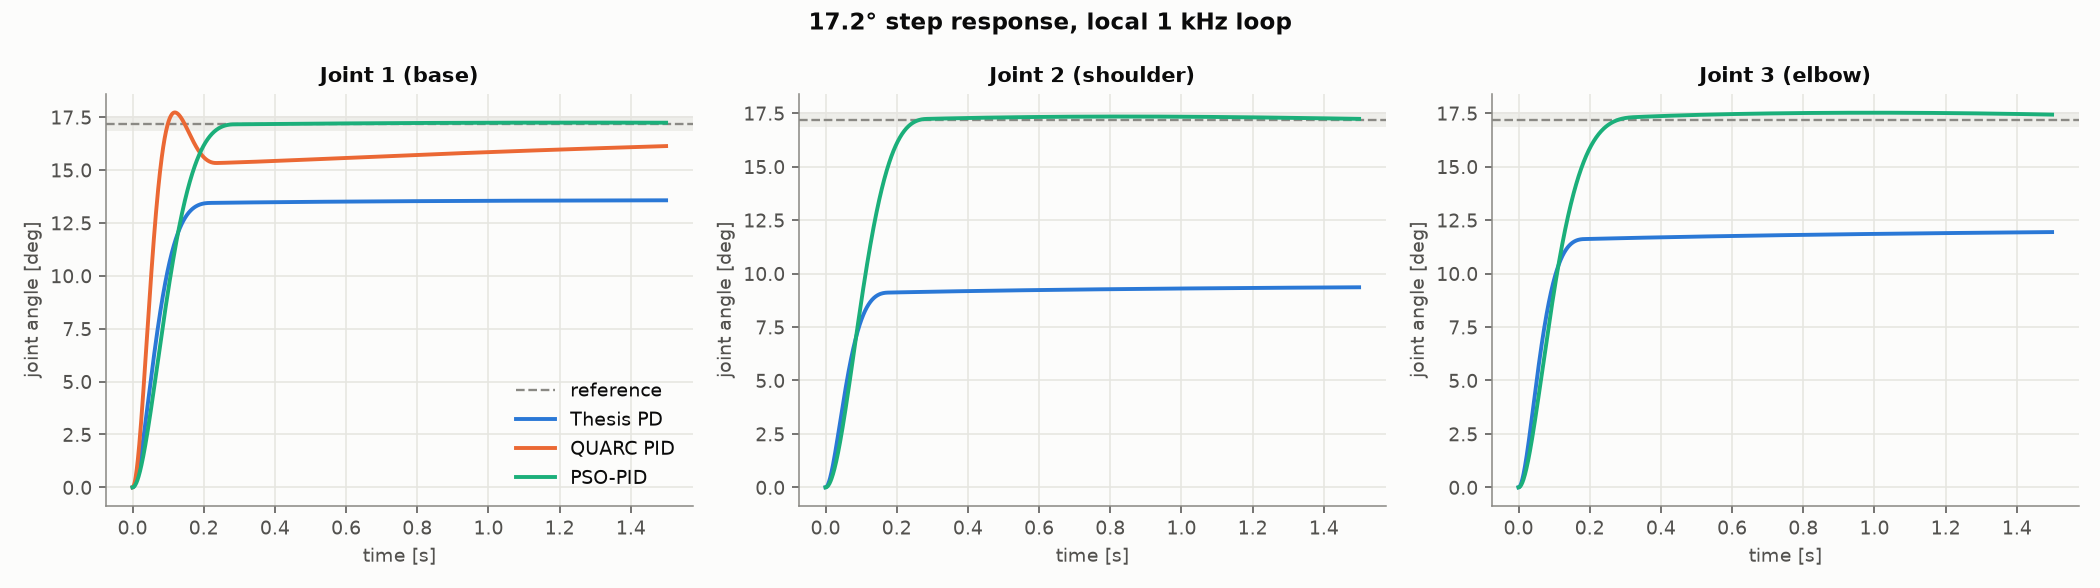
\includegraphics[width=\linewidth]{pso_step_local.png}
\caption{$17.2^\circ$ step responses with a local $1\,\mathrm{kHz}$ loop. The grey band is the $\pm2\,\%$
settling band.}
\label{fig:step_local}
\end{figure}

\begin{figure}[H]
\centering
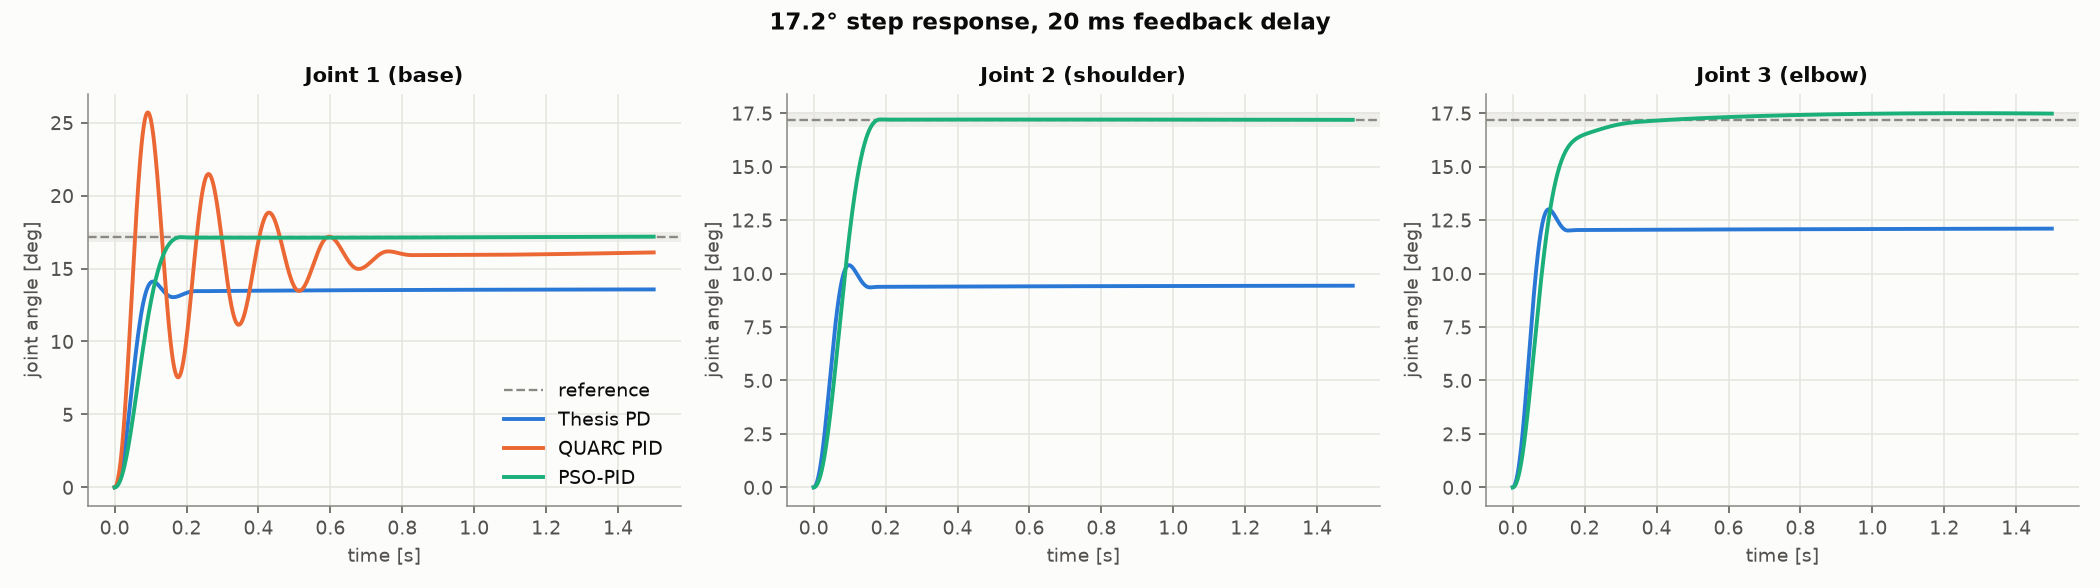
\includegraphics[width=\linewidth]{pso_step_udp.png}
\caption{The same steps with the feedback delayed by one UDP period ($20\,\mathrm{ms}$).}
\label{fig:step_udp}
\end{figure}

\begin{table}[H]
\centering
\small
\begin{tabular}{llrrrrr|rrrr}
\toprule
 & & \multicolumn{5}{c|}{local 1 kHz loop} & \multicolumn{4}{c}{20 ms feedback delay}\\
Controller & J & OS [\%] & $t_s$ [ms] & $e_{ss}$ [$^\circ$] & ITAE & cost & OS [\%] & $t_s$ [ms] & $e_{ss}$ [$^\circ$] & cost\\
\midrule
Thesis PD & 1 & 0.0 & $>$1499 & 3.62 & 0.2415 & 4.573 & 0.0 & $>$1499 & 3.62 & 4.566\\
          & 2 & 0.0 & $>$1499 & 7.84 & 0.5179 & 8.130 & 0.0 & $>$1499 & 7.76 & 8.048\\
          & 3 & 0.0 & $>$1499 & 5.26 & 0.3514 & 5.963 & 0.0 & $>$1499 & 5.09 & 5.800\\
QUARC PID & 1 & 3.1 & $>$1499 & 1.08 & 0.0885 & 2.546 & 49.5 & $>$1499 & 1.11 & 3.555\\
\textbf{PSO-PID} & 1 & 0.3 & 232 & 0.05 & 0.0092 & 0.303 & 0.0 & 158 & 0.01 & 0.187\\
                 & 2 & 0.9 & 231 & 0.06 & 0.0143 & 0.340 & 0.1 & 159 & 0.00 & 0.179\\
                 & 3 & 1.9 & 244 & 0.26 & 0.0255 & 0.535 & 1.8 & 264 & 0.30 & 0.556\\
\bottomrule
\end{tabular}
\caption{Step-response metrics. ``$>$1499'' means the response never entered the $\pm2\,\%$ band within
$1.5\,\mathrm{s}$.}
\label{tab:step}
\end{table}

\begin{itemize}
  \item \textbf{Thesis PD} stops at about $13.6^\circ$, $9.4^\circ$ and $12^\circ$ instead of $17.2^\circ$. At rest
        a PD can only balance the bias torque with a position error, $e_{ss} = b_i/K_{p,i}$, which gives
        $3.6^\circ$, $7.7^\circ$ and $5.0^\circ$, in agreement with the simulation.
  \item \textbf{QUARC PID} (joint 1) slowly removes most of the error, but with $20\,\mathrm{ms}$ of delay it
        overshoots by $49.5\,\%$ and rings for almost a second, because its delay margin is only
        $23.3\,\mathrm{ms}$.
  \item \textbf{PSO-PID} reaches the target in $0.16$--$0.26\,\mathrm{s}$ with at most $1.9\,\%$ overshoot and a
        steady-state error of $0.3^\circ$ or less, in both scenarios. In the local loop its ITAE is
        $14$--$36$ times lower than the PD's. On joints 1 and 2 it even scores slightly better with the delay than without it,
        because it was optimised for the average of both scenarios.
\end{itemize}

\subsection{Frequency response}

\begin{figure}[H]
\centering
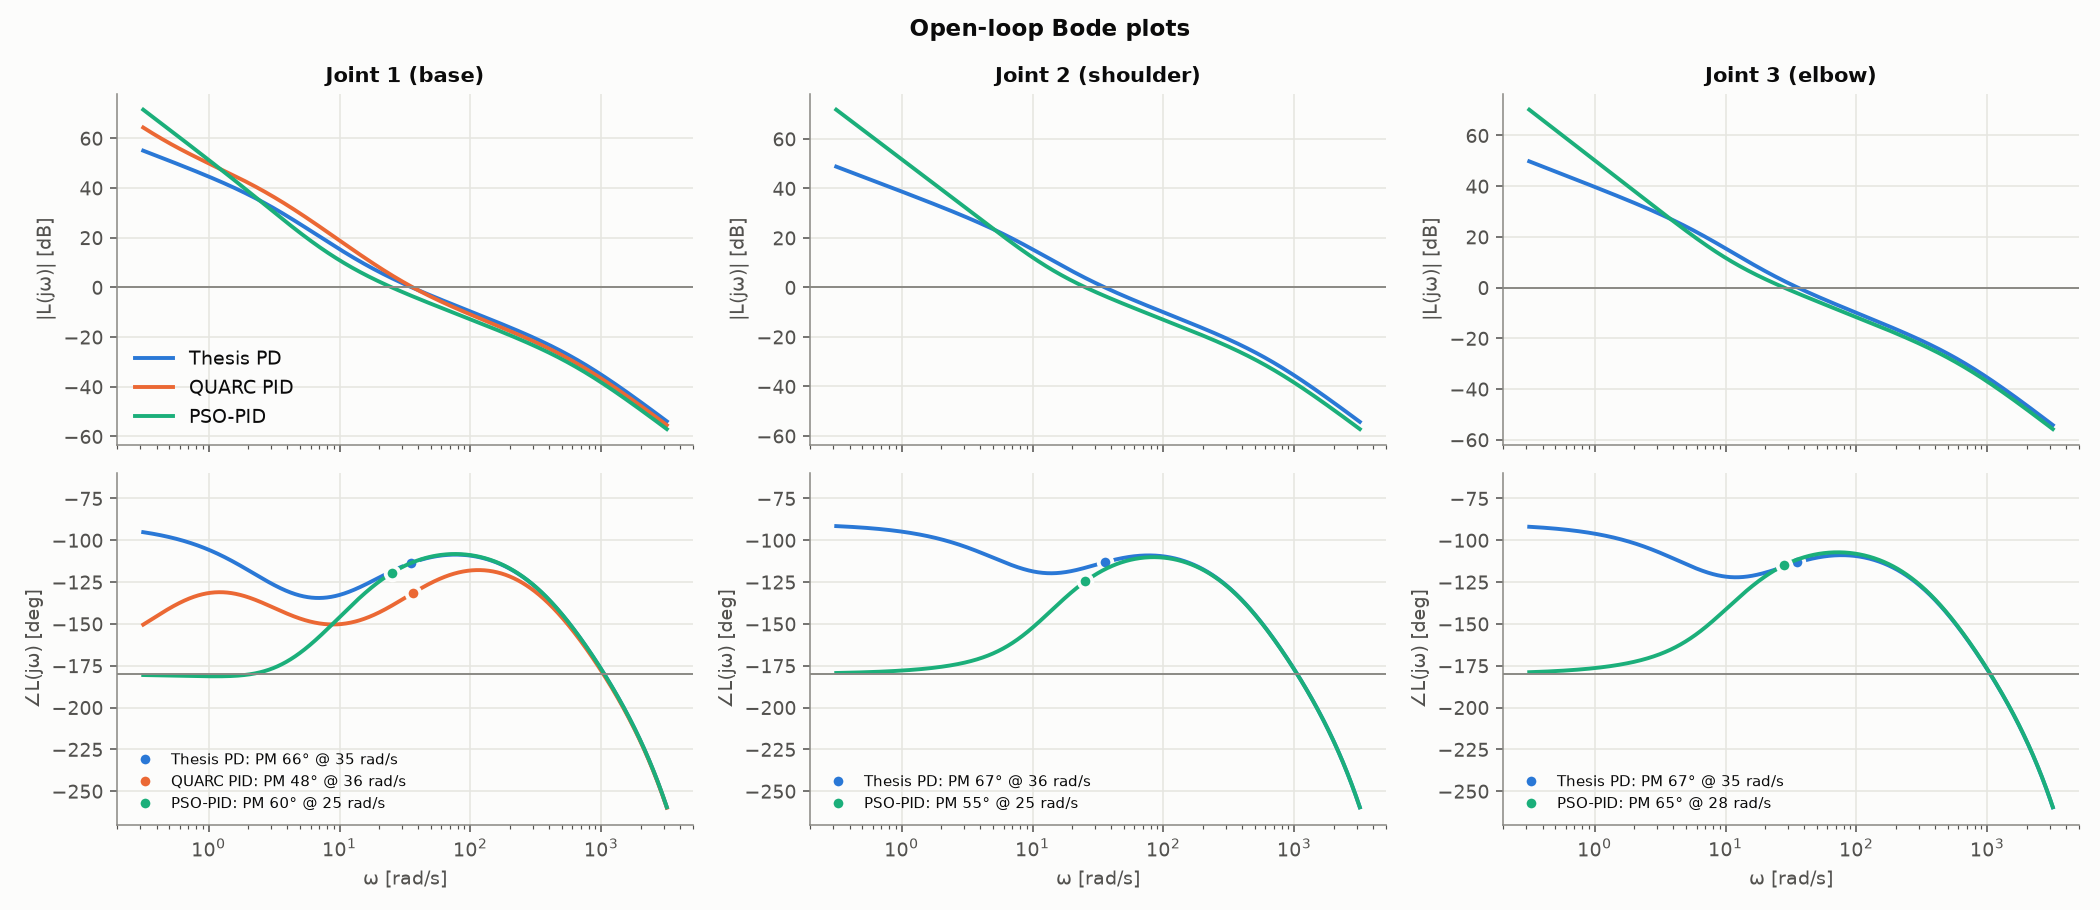
\includegraphics[width=\linewidth]{pso_bode.png}
\caption{Open-loop Bode plots. The dots mark the gain crossover and the phase margin.}
\label{fig:bode}
\end{figure}

The PSO loops contain two integrators (plant and controller), so at low frequency their gain is much higher
than the PD's and their phase starts at $-180^\circ$ (Figure~\ref{fig:bode}). The high low-frequency gain is
what rejects the constant gravity and friction torque. Near the crossover the derivative term lifts the
phase to between $-115^\circ$ and $-125^\circ$, which provides the $56$--$65^\circ$ phase margin.

\subsection{Robustness to delay}

\begin{figure}[H]
\centering
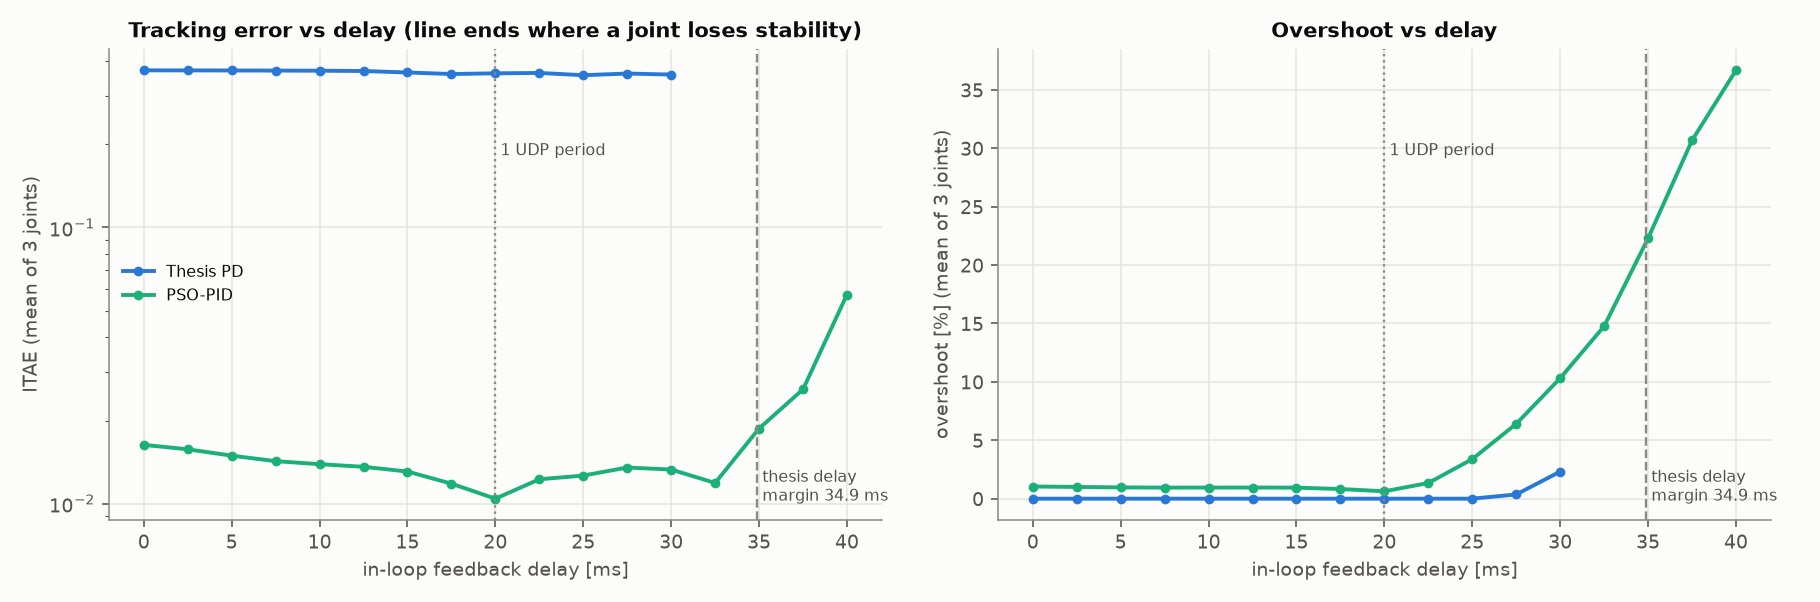
\includegraphics[width=\linewidth]{pso_delay_sweep.png}
\caption{ITAE (left, log scale) and overshoot (right), averaged over the three joints, as the feedback delay
grows. Each line ends at the last delay for which all three joints are stable.}
\label{fig:delay}
\end{figure}

In the delay sweep (Figure~\ref{fig:delay}) the thesis PD first loses stability at $32.5\,\mathrm{ms}$,
right at its predicted delay margin. The reference PSO design stays stable up to $40\,\mathrm{ms}$ and first
fails at $42.5\,\mathrm{ms}$. Wherever both are stable (up to $30\,\mathrm{ms}$) its ITAE is $20$ to $35$
times lower than the PD's, and its overshoot stays around $1\,\%$ up to one UDP period before rising quickly
beyond $25\,\mathrm{ms}$. As the seed study showed, other PSO runs guarantee at least the required
$30\,\mathrm{ms}$ but usually not much more.

\subsection{Validation task: seam welding}

\paragraph{Kinematics.} To judge the controllers on a realistic industrial path, the tool must follow a
Cartesian trajectory, which requires the kinematics of the arm ($L_1 = L_2 = 0.131\,\mathrm{m}$,
\file{src/kinematics.py}). The forward kinematics are
\begin{equation}
\rho = L_1\cos q_2 + L_2\cos(q_2 + q_3),\quad x = \rho\cos q_1,\quad y = \rho\sin q_1,\quad
z = -L_1\sin q_2 - L_2\sin(q_2 + q_3),
\end{equation}
and the closed-form elbow-up inverse kinematics are $q_1 = \operatorname{atan2}(y, x)$,
$\cos q_3 = D = (\rho^2 + z^2 - L_1^2 - L_2^2)/(2L_1L_2)$, $q_3 = \operatorname{atan2}(+\sqrt{1-D^2}, D)$ and
$q_2 = \operatorname{atan2}(-z, \rho) - \operatorname{atan2}(L_2\sin q_3, L_1 + L_2\cos q_3)$. Every target is
checked against a safety shell $0.05 \le \|\bm p\| \le 0.25\,\mathrm{m}$ with a maximum jump of
$0.15\,\mathrm{m}$ between consecutive targets.

\paragraph{Trajectory.} The seam is a $12\,\mathrm{cm}$ straight line along $y$, centred at
$(0.15, 0, -0.04)\,\mathrm{m}$, travelled in $4\,\mathrm{s}$ with a quintic time law (zero velocity and
acceleration at both ends). A $3\,\mathrm{mm}$, $2\,\mathrm{Hz}$ sinusoidal weave across the seam, faded in and
out, imitates the motion of a welding torch. The joint references are sent at $50\,\mathrm{Hz}$, as over UDP,
and a $1.5\,\mathrm{s}$ dwell at the start pose lets each controller settle before the torch moves.

\begin{figure}[H]
\centering
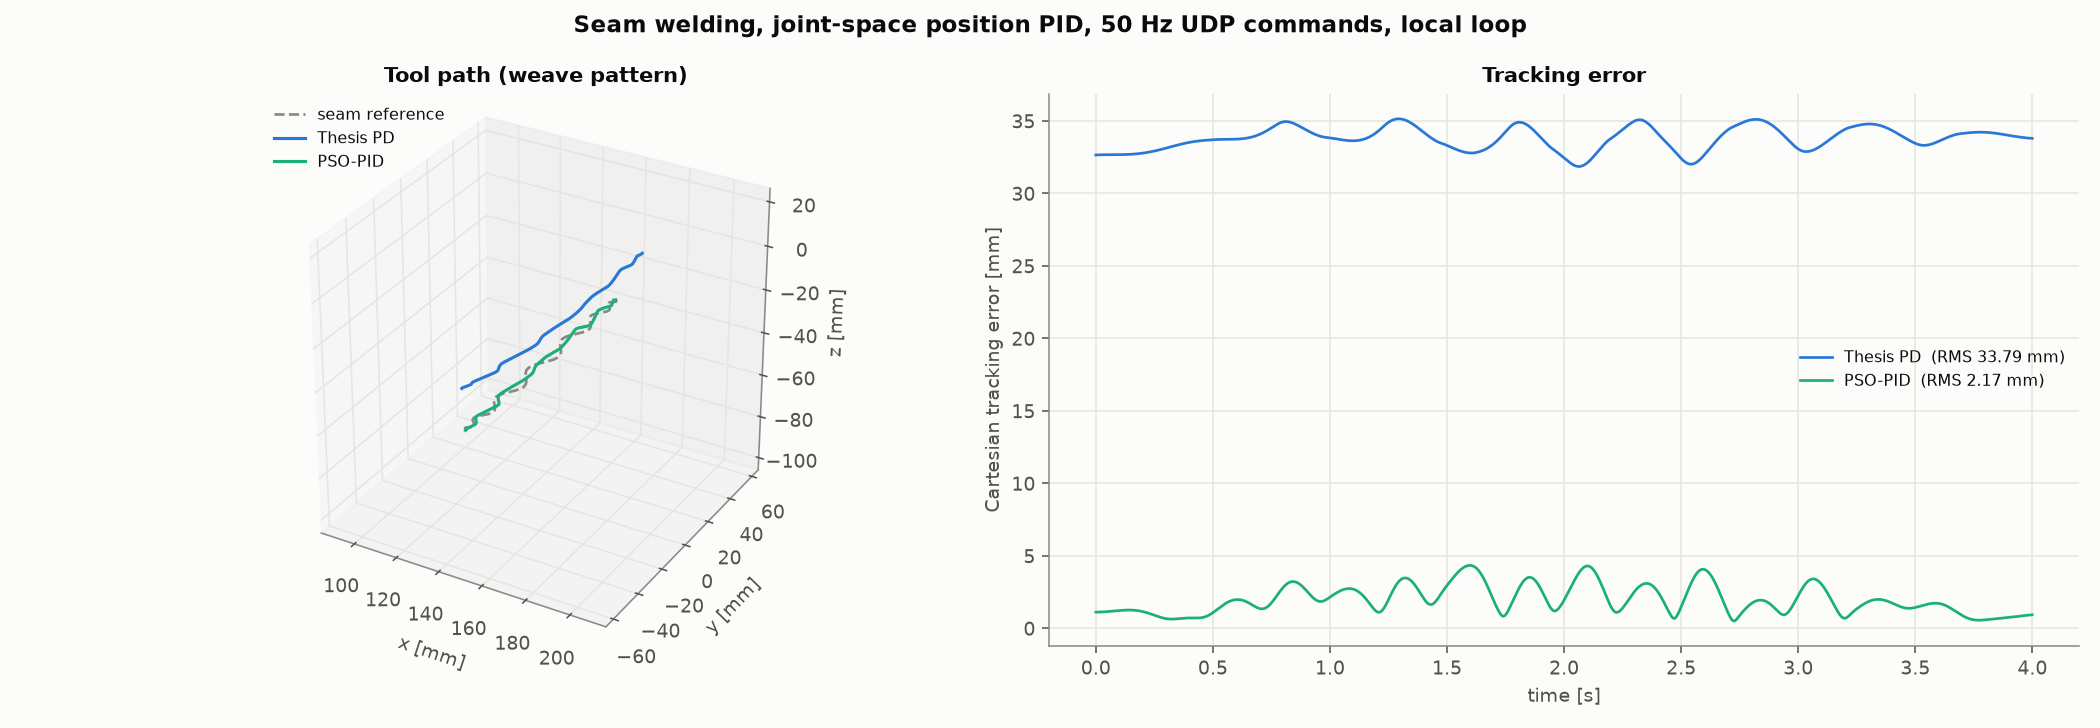
\includegraphics[width=\linewidth]{pso_seam_local.png}
\caption{Seam welding with joint-space position control, local loop. Left: 3-D tool path in millimetres with
equal axis scaling. Right: Cartesian tracking error.}
\label{fig:seam_local}
\end{figure}

\begin{figure}[H]
\centering
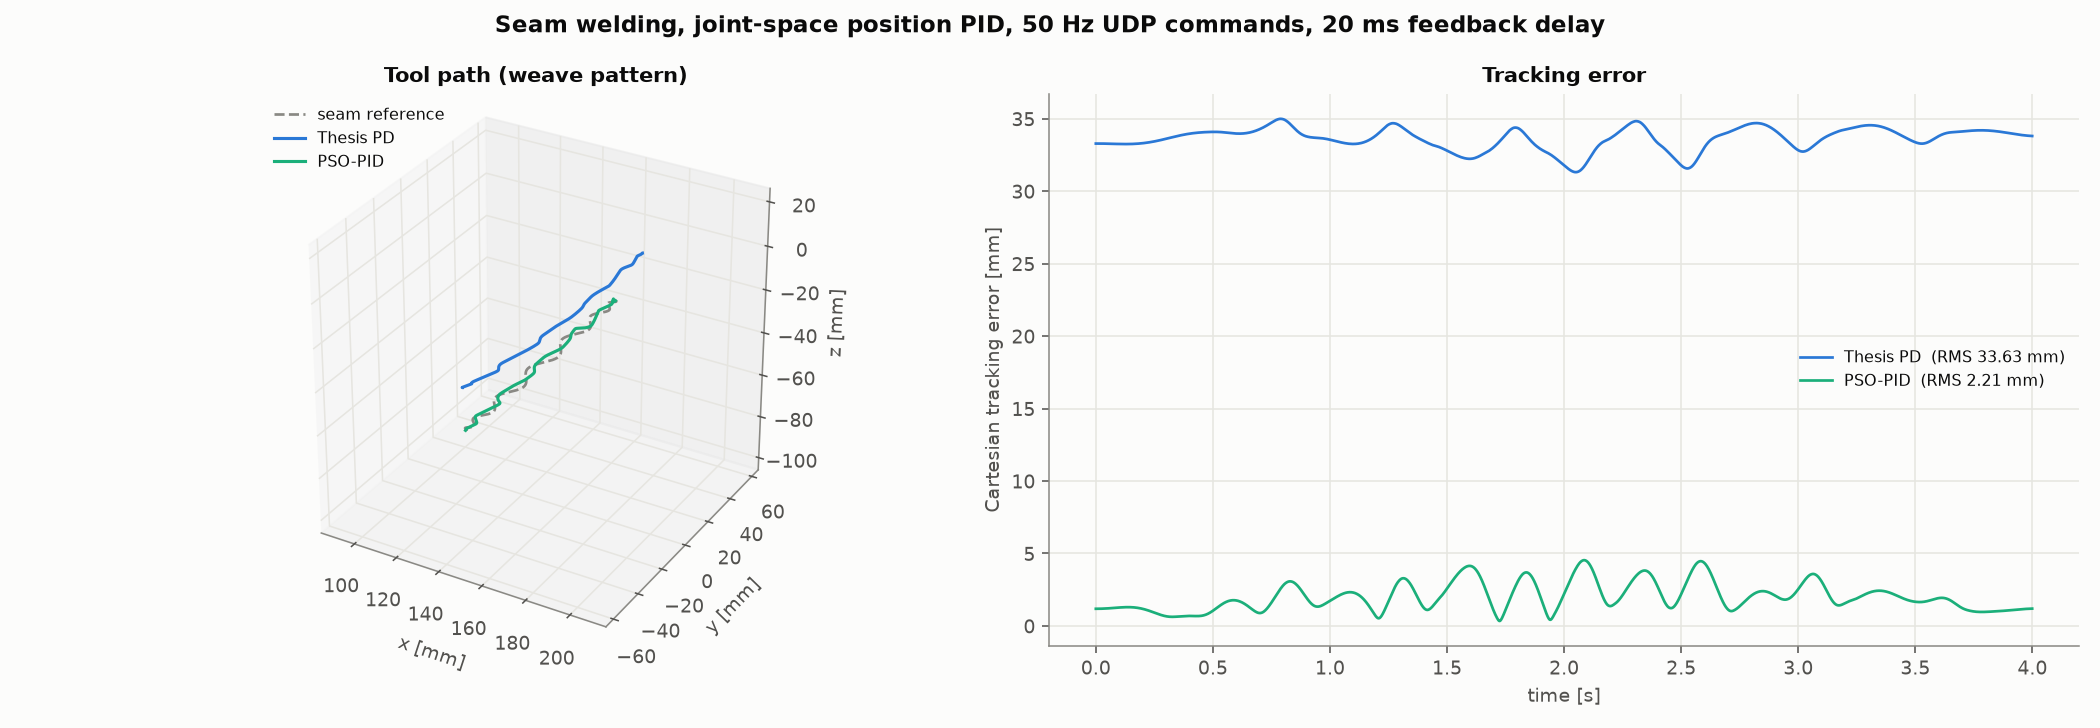
\includegraphics[width=\linewidth]{pso_seam_udp.png}
\caption{The same task with a $20\,\mathrm{ms}$ feedback delay.}
\label{fig:seam_udp}
\end{figure}

With the thesis PD the torch runs parallel to the seam but about $3.4\,\mathrm{cm}$ away from it: the joint
offsets $b_i/K_{p,i}$ become a constant Cartesian offset larger than the whole weave. With the PSO gains
the error drops to $2.17\,\mathrm{mm}$ RMS, a $15$-fold improvement, and the path follows the weave. The
remaining error peaks twice per weave cycle, where the reference changes direction fastest. A
$20\,\mathrm{ms}$ delay barely changes the result ($2.21\,\mathrm{mm}$).

\subsection{Second application: PSO-tuned task-space velocity control}
\label{sec:taskspace}

PSO is not tied to one controller structure. It was also used to tune the inner loops of a
\emph{task-space velocity controller}, which closes the outer loop in Cartesian space:
\begin{equation}
\bm v_{\mathrm{cmd}} = \dot{\bm x}_{\mathrm{ref}} + K_x\left(\bm x_{\mathrm{ref}} - \bm x\right),\qquad
\dot{\bm q}_{\mathrm{ref}} = J^\top\!\left(JJ^\top + \lambda^2 I\right)^{-1}\bm v_{\mathrm{cmd}},\qquad
\tau_i = \mathrm{PID}_{\mathrm{vel},i}\!\left(\dot q_{\mathrm{ref},i} - \dot q_i\right),
\end{equation}
with $K_x = 20\,\mathrm{s^{-1}}$ and $J(\bm q)$ the analytic Jacobian. The damped least-squares inverse, with
$\lambda$ adapted between $0.01$ and $0.05$ according to the smallest singular value of $J$, stays bounded
near singular poses. The three velocity PIDs were tuned with the same PSO and cost function
(\code{--loop velocity}, a $1\,\mathrm{rad/s}$ velocity step, the bounds of Table~\ref{tab:bounds}, no seed
design). PSO reached a cost of $0.468$ with
\begin{gather*}
K_p = [0.1528,\ 0.1132,\ 0.0445],\qquad K_i = [2.4033,\ 2.4079,\ 0.8947],\\
K_d = [0.00114,\ 0.00062,\ 0.00022].
\end{gather*}

\begin{figure}[H]
\centering
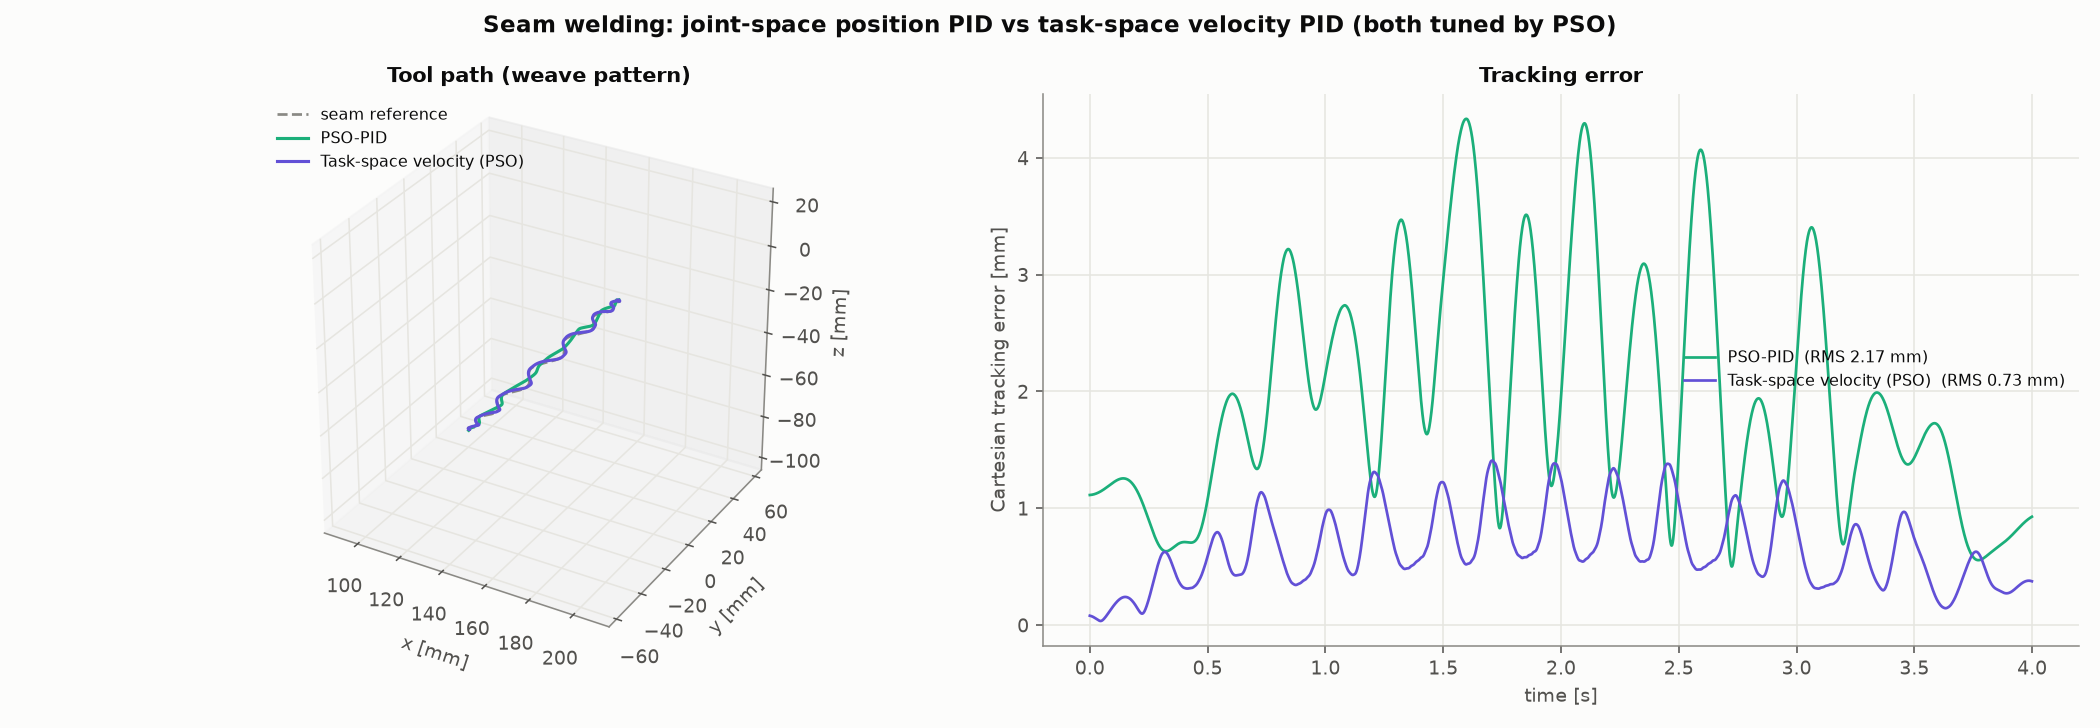
\includegraphics[width=\linewidth]{pso_seam_task_velocity.png}
\caption{Seam welding with the PSO-tuned joint-space position PID and with the PSO-tuned task-space
velocity PID.}
\label{fig:seam_tv}
\end{figure}

\begin{table}[H]
\centering
\begin{tabular}{lccc}
\toprule
Controller & Loop delay [ms] & RMS error [mm] & Max error [mm]\\
\midrule
Thesis PD (joint space) & 0  & 33.787 & 35.140\\
Thesis PD (joint space) & 20 & 33.634 & 34.993\\
PSO-PID (joint space)   & 0  & 2.174  & 4.333\\
PSO-PID (joint space)   & 20 & 2.214  & 4.539\\
PSO velocity PID (task space) & 0 & \textbf{0.728} & \textbf{1.407}\\
\bottomrule
\end{tabular}
\caption{Cartesian tracking error on the seam-welding path.}
\label{tab:seam}
\end{table}

The task-space controller cuts the error by another factor of three, to $0.73\,\mathrm{mm}$ RMS
(Figure~\ref{fig:seam_tv}, Table~\ref{tab:seam}). Its outer loop corrects the tool position directly, and
the velocity feedforward $\dot{\bm x}_{\mathrm{ref}}$ anticipates the weave instead of waiting for an error
to build up.

%=====================================================================================================
\section{Discussion}
\label{sec:discussion}
%=====================================================================================================

\paragraph{What PSO discovered.} Without any knowledge of control theory, the swarm arrived at a design a
control engineer would recognise: integral action to cancel the constant disturbance, a lower crossover
frequency to gain delay margin, and enough derivative action to keep the phase margin above $55^\circ$. It
found this in the first few iterations and spent the rest of the run refining it.

\paragraph{Strengths of PSO for this problem.}
\begin{itemize}[nosep]
  \item It handled a cost that is discontinuous at the stability boundary and dominated by penalties in most
        of the search space (every one of the 29 random initial designs was unstable).
  \item It was reliable: ten seeds out of ten improved the thesis design by a factor of $17$ to $24$.
  \item It is cheap: $1830$ simulations, under half a minute, because the whole swarm is simulated at once.
  \item The same optimiser and cost function tuned a different controller (the task-space velocity loops)
        without modification.
\end{itemize}

\paragraph{Limitations.}
\begin{itemize}
  \item \textbf{Premature convergence.} The global-best topology made the swarm collapse to a diversity of
        $0.003$. At that point it can only refine, not explore. The spread of final costs between seeds
        ($0.77$--$1.08$) shows that different runs end in different parts of a broad valley.
  \item \textbf{The swarm optimises exactly what it is told.} Delay robustness beyond the $30\,\mathrm{ms}$
        floor is not rewarded, so most runs stop just above it. Requirements must be written into the cost
        function.
  \item \textbf{Weights are design choices.} The weights of \eqref{eq:cost} express one trade-off between
        accuracy, speed, overshoot and torque. Other weights would lead to other, equally valid designs.
  \item \textbf{Simplified model.} The joints are decoupled, gravity is a constant bias, and the network is a
        pure delay without jitter or packet loss. The gains must be validated on the QUARC hardware, starting
        with reduced values.
\end{itemize}

\paragraph{Possible improvements.} Running several seeds and keeping the best (seed 2 reached $0.77$);
a local-best topology or a restart when the diversity collapses; more iterations, since the curves still
decrease slightly at iteration 60; raising the delay-margin floor or adding a $30\,\mathrm{ms}$ scenario if
more delay tolerance is required; and tuning on the real robot, using the simulated optimum as the seed
particle.

%=====================================================================================================
\section{How to run the project}
\label{sec:run}
%=====================================================================================================

\subsection{Requirements}

\begin{itemize}[nosep]
  \item Python 3.9 or newer (tested with Python 3.14 on Windows);
  \item the packages \code{numpy}, \code{matplotlib}, \code{pyyaml} and, for the tests, \code{pytest};
  \item a LaTeX distribution (TeX Live or MiKTeX) only to rebuild this PDF.
\end{itemize}
Open a terminal in the project folder (the folder that contains \file{pyproject.toml}) and install the
packages once:
\begin{lstlisting}
pip install numpy matplotlib pyyaml pytest
\end{lstlisting}
On Windows, if \code{python} is not recognised, use \code{py} instead. All commands below are run from the
project folder.

\subsection{Step 1: tune the gains with PSO}

\begin{lstlisting}
python scripts/tune_joint_pid.py --method pso
\end{lstlisting}
This runs the PSO of Algorithm~\ref{alg:pso} on the nine position-loop gains with seed 0 and prints its
progress:
\begin{lstlisting}[basicstyle=\ttfamily\footnotesize]
=== PSO | mode=full | loop=position ===
  [PSO joints [1, 2, 3]] iter   0  best cost 18.5395
  [PSO joints [1, 2, 3]] iter  10  best cost 5.0894
  ...
  [PSO joints [1, 2, 3]] iter  59  best cost 1.0499
  done in 13.7 s, 1830 evaluations, cost 1.0499
  joint 1: Kp=1.0621  Ki=3.3516  Kd=0.0691   PM=60.4 deg  wc=25.0 rad/s  delay margin=42.2 ms
  joint 2: Kp=1.1000  Ki=6.6117  Kd=0.0474   PM=55.6 deg  wc=25.4 rad/s  delay margin=38.1 ms
  joint 3: Kp=0.4078  Ki=1.8709  Kd=0.0231   PM=65.1 deg  wc=28.0 rad/s  delay margin=40.6 ms
\end{lstlisting}
It writes the gains to \file{results/gains_position.json} and plots
\file{results/convergence_position.png} and \file{results/population_pso_position.png}. Useful options:
\begin{lstlisting}[basicstyle=\ttfamily\footnotesize]
python scripts/tune_joint_pid.py --method pso --seed 2             # another random seed
python scripts/tune_joint_pid.py --method pso --iterations 100     # longer run
python scripts/tune_joint_pid.py --method pso --mode per-joint     # three 3-gain searches
python scripts/tune_joint_pid.py --method pso --loop velocity      # velocity-loop gains
\end{lstlisting}
The velocity-loop run writes \file{results/gains_velocity.json}, which the task-space controller uses.

\subsection{Step 2: evaluate the tuned controller}

\begin{lstlisting}
python scripts/compare_baselines.py
\end{lstlisting}
This loads the stored gains and runs every experiment of Section~\ref{sec:results}: step responses, Bode
plots, delay sweep and seam welding. It writes the figures to \file{results/} and a table of all metrics to
\file{results/summary.md}. This script also includes the genetic algorithm in its plots (and tunes it first
if its gains are missing). The PSO-only figures of this document come from the next step.

\subsection{Step 3: regenerate the figures of this document}

\begin{lstlisting}
python docs/make_pso_figures.py                 # 10 seeds, about 3-5 minutes
python docs/make_pso_figures.py --seeds 3       # quicker
\end{lstlisting}
This reruns PSO with seed 0 (and checks that it reproduces \file{results/gains_position.json}), records the
swarm diversity, the unstable share and the global-best trajectory, repeats the run for the other seeds and
writes every figure of Sections~\ref{sec:behaviour} and~\ref{sec:results} to \file{docs/figures/}, together
with the numbers in \file{docs/figures/pso_study.json}.

\subsection{Step 4: build this PDF}

\begin{lstlisting}
cd docs
pdflatex project_documentation.tex
pdflatex project_documentation.tex
\end{lstlisting}
The second run fills in the table of contents and the cross-references. For Overleaf, upload
\file{project_documentation.tex} together with the \file{figures} folder.

\subsection{Step 5: run the tests}

\begin{lstlisting}
python -m pytest
\end{lstlisting}
The 24 tests (about 5 seconds) check the kinematics, the dynamics, the thesis stability margins, the
behaviour under delay, the torque saturation, and that a short PSO run halves the cost of the thesis PD,
never lets its best cost increase and respects the bounds.

\subsection{Changing the PSO settings}

All settings are in \file{config/robot_params.yaml}; no code needs to change:
\begin{itemize}[nosep]
  \item \code{optimization.pso}: swarm size, iterations, $w_{\mathrm{start}}$, $w_{\mathrm{end}}$, $c_1$,
        $c_2$, velocity clamp (Table~\ref{tab:psoparams});
  \item \code{optimization.bounds}: the search box of each gain;
  \item \code{optimization.weights}, \code{pm_min_deg}, \code{dm_min}: the fitness function;
  \item \code{optimization.scenario_delays}: the delays the cost is averaged over.
\end{itemize}
After a change, rerun steps 1 to 3.

\appendix

%=====================================================================================================
\section{Repository layout}
%=====================================================================================================

\begin{table}[H]
\centering
\small
\begin{tabularx}{\linewidth}{@{}>{\raggedright\arraybackslash}p{4.8cm}X@{}}
\toprule
\textbf{Path} & \textbf{Content}\\
\midrule
\file{src/optimizers/pso.py} & The PSO optimiser (Section~\ref{sec:pso}).\\
\file{src/optimizers/__init__.py} & \code{OptimizationResult}: best solution, histories, swarm snapshots, evaluation count.\\
\file{src/objective.py} & Step metrics, stability margins and the fitness \code{PIDObjective}.\\
\file{src/dynamics.py} & Joint plant, RK4 integration, closed-loop simulators with delay and 50\,Hz hold.\\
\file{src/controllers.py} & Discrete PID with filtered derivative and anti-windup.\\
\file{src/kinematics.py} & Forward/inverse kinematics, Jacobian, DLS inverse, workspace guard, seam trajectory.\\
\file{src/visualizer.py} & Plotting functions.\\
\file{src/optimizers/ga.py} & Alternative optimiser (genetic algorithm), not covered here.\\
\file{scripts/tune_joint_pid.py} & Command-line tuning (Step 1).\\
\file{scripts/compare_baselines.py} & Evaluation experiments and \file{summary.md} (Step 2).\\
\file{docs/make_pso_figures.py} & PSO analysis and the figures of this document (Step 3).\\
\file{docs/project_documentation.tex} & This document.\\
\file{config/robot_params.yaml} & All parameters (Appendix~\ref{app:config}).\\
\file{tests/} & 24 automated tests.\\
\file{results/} & Tuned gains (JSON), logs, figures and \file{summary.md}.\\
\bottomrule
\end{tabularx}
\caption{Files relevant to the PSO tuning.}
\end{table}

%=====================================================================================================
\section{Configuration reference}
\label{app:config}
%=====================================================================================================

\begin{table}[H]
\centering
\small
\begin{tabularx}{\linewidth}{@{}>{\raggedright\arraybackslash}p{4.9cm}>{\raggedright\arraybackslash}p{3.6cm}X@{}}
\toprule
\textbf{Key} & \textbf{Value} & \textbf{Meaning}\\
\midrule
\multicolumn{3}{@{}l}{\textit{optimization.pso}}\\
\code{swarm_size}, \code{iterations} & 30, 60 & Particles and iterations.\\
\code{w_start}, \code{w_end} & 0.9, 0.4 & Inertia schedule.\\
\code{c1}, \code{c2} & 1.6, 1.6 & Cognitive and social coefficients.\\
\code{v_max_frac} & 0.2 & Velocity clamp as a fraction of each range.\\
\midrule
\multicolumn{3}{@{}l}{\textit{optimization (fitness)}}\\
\code{loop} & position & Default loop to tune.\\
\code{step_amplitude}, \code{duration} & 0.3 rad, 1.5 s & Test step and simulated horizon.\\
\code{scenario_delays} & [0, 0.020] s & Delays averaged in the cost.\\
\code{bounds} & Table~\ref{tab:bounds} & Search box.\\
\code{weights} & ITAE 4, OS 2, $t_s$ 1, $e_{ss}$ 10, torque 0.5 & Weights of the fitness terms.\\
\code{pm_min_deg}, \code{pm_penalty} & 45, 5 & Phase-margin floor and penalty.\\
\code{dm_min}, \code{dm_penalty} & 0.030 s, 5 & Delay-margin floor and penalty.\\
\midrule
\multicolumn{3}{@{}l}{\textit{dynamics, timing, kinematics}}\\
\code{J}, \code{B}, \code{bias}, \code{coulomb} & Table~\ref{tab:plant} & Joint model.\\
\code{coulomb_smoothing} & 0.01 rad/s & Friction smoothing $v_s$.\\
\code{tau_max}, \code{tau_cont} & Table~\ref{tab:plant} & Torque limits.\\
\code{Ts}, \code{T_udp} & 0.001 s, 0.020 s & Control period, UDP period.\\
\code{deriv_cutoff_hz} & 100 & Derivative filter cutoff [Hz].\\
\code{L1}, \code{L2} & 0.131 m & Link lengths.\\
\code{workspace} & 0.05--0.25 m, jump 0.15 m & Safety shell.\\
\code{dls_lambda} & [0.01, 0.05] & DLS damping range.\\
\midrule
\multicolumn{3}{@{}l}{\textit{baselines}}\\
\code{thesis_pd}, \code{quarc_pid_joint1} & Table~\ref{tab:gains} & Thesis reference gains.\\
\bottomrule
\end{tabularx}
\caption{Parameters in \code{config/robot_params.yaml}.}
\end{table}

%=====================================================================================================
\begin{thebibliography}{9}
\bibitem{gavan2026} Găvan, \emph{Omni Bundle -- Haptic Device's Industrial Approach}, bachelor's thesis, 2026, Section~7.9.
\bibitem{kennedy1995} J.~Kennedy and R.~Eberhart, ``Particle swarm optimization,'' in \emph{Proc.\ IEEE International Conference on Neural Networks}, vol.~4, pp.~1942--1948, 1995.
\bibitem{shi1998} Y.~Shi and R.~Eberhart, ``A modified particle swarm optimizer,'' in \emph{Proc.\ IEEE International Conference on Evolutionary Computation}, pp.~69--73, 1998.
\bibitem{eberhart2000} R.~C.~Eberhart and Y.~Shi, ``Comparing inertia weights and constriction factors in particle swarm optimization,'' in \emph{Proc.\ IEEE Congress on Evolutionary Computation}, pp.~84--88, 2000.
\bibitem{clerc2002} M.~Clerc and J.~Kennedy, ``The particle swarm -- explosion, stability, and convergence in a multidimensional complex space,'' \emph{IEEE Transactions on Evolutionary Computation}, vol.~6, no.~1, pp.~58--73, 2002.
\bibitem{poli2009} R.~Poli, ``Mean and variance of the sampling distribution of particle swarm optimizers during stagnation,'' \emph{IEEE Transactions on Evolutionary Computation}, vol.~13, no.~4, pp.~712--721, 2009.
\end{thebibliography}

\end{document}
